\documentclass[letterpaper,11pt]{article}

\usepackage[utf8]{inputenc}
\usepackage[spanish]{babel}
\usepackage[
    letterpaper,
    top=1.7cm,
    bottom=2cm,
    left=2cm,
    right=2cm
]{geometry}

\usepackage{graphicx}
\usepackage{fancyhdr}
\usepackage[table,xcdraw]{xcolor}
\usepackage{tikz}
\usetikzlibrary{shapes.geometric, shapes.symbols, arrows, positioning, fit, backgrounds, calc, babel, decorations.pathreplacing}
\usepackage{ifpdf}
\usepackage[cmex10]{amsmath}
\usepackage{amssymb}
\usepackage{amsfonts}
\usepackage{float}
\usepackage{siunitx}
\usepackage{listings}
\usepackage{hyperref}
\usepackage{booktabs}
\usepackage{url}
\usepackage{titlesec}
\usepackage[export]{adjustbox}
\usepackage{parskip}
\usepackage[numbers]{natbib}
\usepackage{ragged2e}
\usepackage{array}
\usepackage{longtable}
\usepackage{multirow}
\usepackage{pgfplots}
\pgfplotsset{compat=1.17}
\usepackage{makecell}

\newcolumntype{L}[1]{>{\RaggedRight\arraybackslash}p{#1}}

\hypersetup{colorlinks=false,bookmarksopen=true,linkbordercolor={1 1 1}}
\newcommand{\rfigura}[1]{Fig.\,\ref{#1}}
\newcommand{\rtabla}[1]{Tabla \ref{#1}}

\newcommand{\Curso}{IEE2913 --- Diseño Eléctrico (Capstone)}
\newcommand{\TituloInforme}{Informe de Avance 2 (25\,\%)}
\newcommand{\NumeroGrupo}{10}
\newcommand{\NombreProyecto}{SupaClock: Wearable Biométrico Modular}
\newcommand{\Integrantes}{Tomás Avendaño, Benjamín Sepúlveda, Pablo Uribe}
\newcommand{\FechaEntrega}{27 de abril de 2026}

\lstset{
  basicstyle=\ttfamily\small,
  breaklines=true,
  breakatwhitespace=true,
  postbreak=\mbox{\textcolor{red}{$\hookrightarrow$}\space},
  captionpos=b,
  frame=single,
  numbers=left,
  numberstyle=\tiny\color{gray},
  language=C,
  keywordstyle=\color{blue}\bfseries,
  commentstyle=\color{gray}\itshape,
  stringstyle=\color{red!70!black},
  showstringspaces=false,
  inputencoding=utf8,
  extendedchars=true,
  literate=
    {á}{{\'a}}1 {é}{{\'e}}1 {í}{{\'i}}1 {ó}{{\'o}}1 {ú}{{\'u}}1
    {Á}{{\'A}}1 {É}{{\'E}}1 {Í}{{\'I}}1 {Ó}{{\'O}}1 {Ú}{{\'U}}1
    {ñ}{{\~n}}1 {Ñ}{{\~N}}1 {ü}{{\"u}}1 {Ü}{{\"U}}1
    {¿}{{?`}}1 {¡}{{!`}}1 {°}{{$^\circ$}}1
}

\begin{document}

% =========== Encabezado ===========
\noindent
\begin{minipage}[c]{0.12\textwidth}
    
\includegraphics[width=0.9\linewidth]{logo.pdf}
\end{minipage}
\hfill
\begin{minipage}[c]{0.68\textwidth}
    \small
    PONTIFICIA UNIVERSIDAD CATÓLICA DE CHILE\\
    ESCUELA DE INGENIERÍA\\
    Departamento de Ingeniería Eléctrica\\
    \Curso
\end{minipage}
\hfill
\begin{minipage}[c]{0.15\textwidth}
    \raggedleft
    \small
    Grupo \NumeroGrupo
\end{minipage}

\vspace{0.4cm}

\begin{center}
    {\Large \textbf{\TituloInforme}}\\[0.4cm]
\end{center}

\noindent\textbf{Proyecto:} \NombreProyecto\\
\textbf{Integrantes:} \Integrantes\\
\textbf{Fecha:} \FechaEntrega

\hrule

\vspace{0.5cm}

\renewcommand{\contentsname}{Índice}
\tableofcontents
\listoffigures
\listoftables
\newpage

% =====================================================
\section{Introducción al estado actual del proyecto}
% =====================================================
Este documento detalla el estado actual del desarrollo del proyecto \textit{SupaClock},
dando continuidad al diseño establecido en el reporte preliminar del 7 de abril de
2026. La motivación, los requerimientos técnicos y el diagrama de bloques de alto nivel descritos en aquel
documento se mantienen vigentes, por lo que en este informe \textbf{no se reproducen}, sino que se
referencian. El presente documento se estructura en torno a cinco ejes fundamentales:
diagrama de bloques de bajo nivel \textit{actualizado}, planificación contrastada con el estado real
del proyecto, análisis de impacto socioeconómico y de estándares aplicables, modelos y simulaciones
que respaldan las decisiones de diseño, set-up final de pruebas y un diseño de pruebas preliminar
(sección que se incorpora en este reporte para complementar la planificación original).
Adicionalmente, en la \textbf{sección de Implementación y resultados} se documentan todos los bloques
que el equipo logró integrar en la iteración actual de desarrollo.

\subsubsection{Resumen ejecutivo del avance.} Actualmente el sistema cuenta con un
\textbf{firmware funcional integrado} que ejerce a las cinco tareas concurrentes bajo FreeRTOS
(IMU + pasos, PPG, Temperatura/Batería, ECG por DMA y GUI LVGL), un \textbf{stack BLE NimBLE}
operativo con tres características GATT, un \textbf{backend Firebase} con Cloud Functions
corriendo Pan-Tompkins en NumPy y un \textbf{esquemático en KiCad} para el prototipo SuperMini.
Los componentes de Machine Learning (CNN 1D para HAR) y la PCB SMD propia están en fases
tempranas y se concentran en los hitos 60\,\% y 90\,\%. La aplicación móvil que actuará como
\textit{gateway} entre el dispositivo y el backend se abordará en iteraciones posteriores y queda fuera del
alcance de este reporte; para la fase de diseño actual, las trazas BLE se validan con un cliente de
escritorio (\texttt{nRF Connect} y un \texttt{ble\_logger.py} propio en Python) que también
escribe directamente en Firestore para verificar el extremo \textit{cloud}.

% =====================================================
\section{Diagrama de bloques de bajo nivel actualizado}
% =====================================================
El diagrama de alto nivel presentado en la \textit{Fig.\,4} de la entrega anterior se mantiene
\textbf{sin modificaciones estructurales}: los siete dominios funcionales (interacción, energía,
sensores, MCU, interfaz local, gateway y backend) y sus interconexiones siguen siendo válidos.
Lo que sí se actualizó es el \textbf{nivel de detalle de bajo nivel}, dado que ahora cada bloque
tiene un grado de implementación cuantificable sobre placa de desarrollo. La \rfigura{fig:lownivel}
muestra el estado vigente, codificando con color el porcentaje de integración y diferenciando con un
borde discontinuo aquellos bloques que aún no están implementados o cuyo paso a la PCB propia
está pendiente.

\begin{figure}[H]
    \centering
    \resizebox{\textwidth}{!}{\begin{tikzpicture}[
    node distance=0.6cm and 0.9cm,
    every node/.style={font=\scriptsize},
    blockOK/.style={rectangle, rounded corners, draw=black!70, very thick, fill=green!22, text width=3.0cm, align=center, minimum height=0.95cm},
    blockPart/.style={rectangle, rounded corners, draw=black!70, very thick, fill=yellow!28, text width=3.0cm, align=center, minimum height=0.95cm},
    blockTodo/.style={rectangle, rounded corners, draw=black!70, very thick, dashed, fill=red!12, text width=3.0cm, align=center, minimum height=0.95cm},
    pcb/.style={rectangle, rounded corners, draw=blue!70, very thick, fill=blue!10, text width=3.0cm, align=center, minimum height=0.95cm},
    energy/.style={rectangle, rounded corners, draw=black!70, very thick, fill=orange!22, text width=3.0cm, align=center, minimum height=0.9cm},
    mcu/.style={rectangle, rounded corners, draw=black, very thick, fill=blue!22, text width=3.6cm, align=center, minimum height=1.4cm, font=\small\bfseries},
    busI2C/.style={->, >=stealth, thick, blue!70!black},
    busSPI/.style={->, >=stealth, thick, violet!80!black},
    adc/.style={->, >=stealth, thick, orange!85!black},
    gpio/.style={->, >=stealth, thick, teal!70!black},
    ble/.style={->, >=stealth, thick, dashed, blue!60},
    pwr/.style={->, >=stealth, thick, red!70},
    legend/.style={rectangle, draw=black!50, fill=white, inner sep=4pt}
]
% ============== ENERGÍA ==============
\node[energy] (usbc)  {USB-C\\\textit{(prototipo)}};
\node[energy, right=of usbc] (bms)   {BMS TP4056 + DW01A\\\textbf{100\%} (módulo)};
\node[energy, right=of bms]  (lipo)  {Bater\'ia LiPo 3.7\,V\\\textbf{100\%} (502030)};
\node[energy, below=of bms]  (ldo)   {LDO ME6211 3.3\,V\\\textbf{100\%} (módulo)};
\node[blockOK, below=of lipo] (fuel) {MAX17048\\\textbf{100\%} (driver listo)};

% ============== MCU ==============
\node[mcu, right=2cm of fuel] (mcu) {ESP32-C3 SuperMini\\FreeRTOS + LVGL 8.4\\\textbf{Funcionando}};

% ============== SENSORES I2C ==============
\node[blockOK, above=of mcu, xshift=3.3cm] (max205) {MAX30205\\\textbf{100\%} \textit{(0x48)}};
\node[blockOK, right=of max205]            (bmi)    {BMI160 IMU\\\textbf{100\%} \textit{(0x68)}};
\node[blockOK, below=of bmi]               (max102) {MAX30102\\\textbf{95\%} HR/SpO\textsubscript{2}};

% ============== ECG (analógico + DMA) ==============
\node[blockOK, below=of max102] (ad8232) {AD8232 + DMA\\\textbf{90\%} \textit{(GPIO0)}};

% ============== INTERFAZ LOCAL ==============
\node[blockOK, left=2.0cm of mcu] (st7789) {ST7789 1.69" IPS\\\textbf{100\%} (LVGL)};
\node[blockOK, above=of st7789]   (btns)   {3 botones GPIO\\\textbf{100\%} (debounce)};
\node[blockPart, below=of st7789] (gui)    {GUI: Home/Bio/ECG/Menu\\\textbf{85\%} (4 pant.)};

% ============== ECOSISTEMA ==============
\node[blockOK, below=2.4cm of mcu, xshift=-0.4cm] (ble) {BLE NimBLE\\\textbf{100\%} (3 GATT chr.)};
\node[blockPart, right=of ble]                     (cli) {Cliente PC testing\\\textbf{60\%} (\texttt{ble\_logger.py})};
\node[blockOK, right=of cli]                       (fb)  {Firebase + Pan-Tompkins\\\textbf{100\%} (Cloud Fn)};
\node[blockTodo, below=of fb]                      (ml)  {TinyML (CNN 1D)\\\textbf{0\%} (rec.\ datos)};
\node[blockTodo, below=of cli]                     (pcb) {PCB SuperMini propia\\\textbf{30\%} (KiCad WIP)};
\node[blockTodo, below=of ble]                     (app) {App m\'ovil (gateway)\\\textbf{0\%} (hito 60\%)};

% ============== Conexiones de potencia ==============
\draw[pwr] (usbc)  -- (bms);
\draw[pwr] (bms)   -- (lipo);
\draw[pwr] (bms)   -- (ldo);
\draw[pwr] (lipo)  -- (fuel);
\draw[pwr] (ldo.east)  -- ++(0.3,0) |- (mcu.west);

% ============== Buses I2C ==============
\draw[busI2C] (max205) -- node[above]{I2C 400\,kHz} (mcu);
\draw[busI2C] (bmi)    -- (mcu);
\draw[busI2C] (max102) -- (mcu);
\draw[busI2C] (fuel)   -- (mcu);

% ============== ECG analógico ==============
\draw[adc] (ad8232) -- node[below, sloped]{ADC1 / DMA 20\,kHz} (mcu);

% ============== SPI display + GPIO botones ==============
\draw[busSPI] (mcu.west) -- node[above]{SPI 80\,MHz} (st7789.east);
\draw[gpio]   (btns)   -- (mcu.north west);

% ============== BLE / cloud ==============
\draw[ble] (mcu)  -- (ble);
\draw[ble] (ble)  -- node[above]{GATT 3 chr.} (cli);
\draw[gpio, ->] (cli) -- node[above]{Wi-Fi/REST} (fb);
\draw[ble, ->, dashed, gray!60] (ble) -- node[left]{futuro} (app);
\draw[ble, ->, dashed, gray!60] (app) -| (fb);

% ============== Leyenda ==============
\node[legend, below=1.6cm of ble, xshift=4cm] (leg) {%
\begin{tabular}{ll}
\textcolor{green!50!black}{$\blacksquare$} Funcionando &
\textcolor{orange!80!black}{$\blacksquare$} Parcial \\
\textcolor{red!70!black}{$\blacksquare$} Pendiente / dependiente &
\textcolor{red!70}{\textbf{$\rightarrow$}} Potencia \\
\textcolor{blue!70!black}{$\rightarrow$} I2C 400\,kHz &
\textcolor{violet!80!black}{$\rightarrow$} SPI 80\,MHz \\
\textcolor{orange!85!black}{$\rightarrow$} ADC/DMA &
\textcolor{blue!60}{$\dashrightarrow$} BLE / Wi-Fi \\
\end{tabular}};
\end{tikzpicture}
}
    \caption{Diagrama de bloques de bajo nivel actualizado del prototipo SupaClock. Cada bloque
    indica el porcentaje de implementación actual. Verde: funcional;
    amarillo: parcial; rojo punteado: pendiente o dependiente de la PCB SMD.}
    \label{fig:lownivel}
\end{figure}

\subsubsection{Cambios respecto del diagrama original.} La estructura general del bus es la misma;
las modificaciones son:
\begin{itemize}
    \item \textbf{Bus I2C}: confirmado a 400\,kHz con cuatro esclavos físicos
    (MAX30102 \texttt{0x57}, MAX30205 \texttt{0x48}, BMI160 \texttt{0x68}, MAX17048 \texttt{0x36}),
    accedido bajo el mutex \texttt{xSensorDataMutex} (FreeRTOS) para serializar las cuatro tareas
    concurrentes que comparten el bus.
    \item \textbf{ADC continuo (ECG)}: el AD8232 ya \textit{no} se concibe como un canal ADC
    \textit{single-shot}; la implementación actual usa el periférico \texttt{adc\_continuous}
    del ESP-IDF a 20\,kHz con DMA, decimando por 40 hacia 500\,Hz para BLE. Esto se justifica en
    la \rfigura{fig:rtos}.
    \item \textbf{Botones}: pasaron de tres a tres botones \textit{con \textit{double-tap} y
    \textit{long-press}} gestionados por \texttt{gpio\_buttons} (debounce SW por
    \texttt{esp\_timer}); el pin de despertar de \textit{deep sleep} se canaliza ahora por
    \texttt{BTN\_SELECT} en lugar de la INT1 del IMU.
    \item \textbf{LVGL}: se confirmó el buffer parcial de 14.4\,KB (240$\times$30 px $\times$ 2\,B);
    el GUI quedó dividido en cuatro pantallas (Home, Bio, ECG, Menú) con navegación por estado.
    \item \textbf{Backend Firebase}: el flujo \textit{dispositivo $\to$ Firestore $\to$ Cloud
    Function \texttt{process\_ecg}} ya está desplegado y se valida con un cliente de
    \textit{testing} en PC; el \textit{gateway} móvil definitivo se construirá en el hito 60\,\%.
    \item \textbf{TinyML}: aún \textit{no} se entrenó el modelo CNN 1D (depende de la
    recolección de datos reales del BMI160 sobre los integrantes); por eso se mantiene como bloque
    pendiente. El contador de pasos \textit{algorítmico} (umbral adaptativo) sí se implementó.
    \item \textbf{PCB SMD propia}: el esquemático en KiCad (\texttt{hardware/PCB\_Prototipo})
    incluye la sección de potencia y los \textit{footprints} importados desde la librería
    Adafruit-MAX17048 y el módulo TP4056; el ruteo del bottom de sensores está pendiente, por
    lo que el bloque se reporta al 30\,\%.
\end{itemize}

\subsubsection{Especificaciones detalladas por bloque.} La \rtabla{tab:specs} consolida las
especificaciones cuantitativas que permiten cerrar el diagrama. La columna ``Estado'' usa
la misma codificación cromática que la \rfigura{fig:lownivel}.

\begin{table}[H]
    \centering
    \caption{Especificaciones de bajo nivel por bloque y estado de implementación.}
    \label{tab:specs}
    \footnotesize
    \begin{tabular}{|L{2.6cm}|L{2.0cm}|L{2.6cm}|L{4.6cm}|L{2.0cm}|}\hline
    \rowcolor{gray!20}\textbf{Bloque} & \textbf{Interfaz} & \textbf{Frecuencia / tasa} & \textbf{Especificación clave} & \textbf{Estado} \\\hline
    AD8232 (ECG)         & ADC1\,/\,DMA      & 20\,kHz $\to$ 500\,Hz (down-sample 40$\times$)  & GPIO0 ADC, ganancia analógica fija 1100, $f_c$\,LP $\sim$40\,Hz   & \cellcolor{green!20}90\,\% \\\hline
    BMI160 (IMU)         & I2C 400\,kHz \texttt{0x68} & ODR 50\,Hz                              & accel $\pm 2$\,g, gyro $\pm 250$\,°/s, FIFO HW, INT1 step counter & \cellcolor{green!20}100\,\% \\\hline
    MAX30102 (PPG)       & I2C 400\,kHz \texttt{0x57} & 100\,sps efect.\ ($N_{avg}=4$)         & RED+IR pulse 411\,$\mu$s, FIFO 32, polling 100\,ms, flush startup  & \cellcolor{green!20}95\,\% \\\hline
    MAX30205 (Temp)      & I2C 400\,kHz \texttt{0x48} & 1\,Hz polling                          & 16-bit, 0.00390625\,°C/LSB, $\pm 0.1$\,°C en rango clínico        & \cellcolor{green!20}100\,\% \\\hline
    MAX17048 (Fuel)      & I2C 400\,kHz \texttt{0x36} & 1\,Hz polling                          & ModelGauge SOC \%, $V_{cell}$\,mV, sin shunt externo               & \cellcolor{green!20}100\,\% \\\hline
    ST7789 (Display)     & SPI 80\,MHz, 4-wire & 30\,FPS LVGL                                  & 240$\times$280 RGB565, DMA \texttt{SPI\_DMA\_CH\_AUTO}, offset Y=20 & \cellcolor{green!20}100\,\% \\\hline
    Botones GPIO         & GPIO IN pull-up   & polling 30\,Hz desde gui\_task                  & 3 botones, 30\,ms debounce, eventos short/long, wake-up sleep      & \cellcolor{green!20}100\,\% \\\hline
    BMS TP4056 + DW01A   & USB-C IN          & --                                              & carga 1\,A ajustable, OVP/OCP/UVP integrado                       & \cellcolor{green!20}100\,\% \\\hline
    LDO ME6211           & 3.3\,V OUT        & --                                              & dropout $\sim$100\,mV @ 100\,mA, $I_Q$\,55\,$\mu$A                 & \cellcolor{green!20}100\,\% \\\hline
    BLE NimBLE           & 2.4\,GHz BLE 5    & MTU 247, conn.\ interval 15\,ms                & 3 chr.: 0xFF01 IMU, 0xFF02 sensores lentos, 0xFF03 ECG raw         & \cellcolor{green!20}100\,\% \\\hline
    GUI LVGL             & SPI                & 30\,FPS                                         & 4 pantallas, navegación 2 botones + auto-switch ECG               & \cellcolor{yellow!25}85\,\% \\\hline
    Cloud Functions      & Firestore trigger & on\_document\_created                          & Pan-Tompkins NumPy, BPM, HRV (SDNN), R-peaks                       & \cellcolor{green!20}100\,\% \\\hline
    TinyML CNN 1D        & TFLite Micro      & 0.5\,Hz inferencia                              & 4 clases HAR, $<$30\,KB flash, $\leq$10\,KB SRAM                   & \cellcolor{red!15}0\,\% \\\hline
    PCB SuperMini propia & 4 capas JLCPCB    & --                                              & sandwich 2 PCBs, ventana óptica PPG, perno M3 ECG                  & \cellcolor{red!15}30\,\% \\\hline
    \end{tabular}
\end{table}

% =====================================================
\section{Planificación actualizada}
% =====================================================

\subsection{Contraste avance esperado vs.\ avance logrado}
La \rtabla{tab:gantt25} contrasta las tareas de la planificación preliminar
con su estado actual. Las filas
en verde indican tareas completadas; las amarillas, tareas en curso; las rojas, tareas
\textit{adelantadas} respecto del cronograma original o tareas nuevas que se incorporaron al
descubrir necesidades de implementación que no estaban en la planificación inicial.

\begin{table}[H]
    \centering
    \caption{Contraste entre actividades planificadas preliminarmente
    y el avance logrado al 27 de abril de 2026.}
    \label{tab:gantt25}
    \footnotesize
    \begin{tabular}{|L{4.0cm}|L{2.4cm}|L{8.0cm}|}\hline
    \rowcolor{gray!20}\textbf{Tarea planificada} & \textbf{Estado} & \textbf{Observaciones} \\\hline
    \cellcolor{green!12} Implementación bloque de energía (BMS + LDO) & \cellcolor{green!20}\bf Completado & Módulo TP4056 + DW01A montado y validado a 4.2\,V; LDO ME6211 entrega 3.30\,V estables. Driver \texttt{max17048} entrega SOC y $V_{cell}$ con 1\,Hz polling. \\\hline
    \cellcolor{green!12} Integración inicial de sensores en bus I2C compartido & \cellcolor{green!20}\bf Completado & Cuatro esclavos en el bus a 400\,kHz, mutex FreeRTOS protege accesos concurrentes desde 4 tareas. Sin colisiones tras 24\,h de operación continua. \\\hline
    \cellcolor{green!12} Pruebas preliminares de adquisición de datos & \cellcolor{green!20}\bf Completado & Cada \texttt{env:test\_*} de PlatformIO valida un sensor de forma aislada; existen 9 entornos de prueba unitarios. \\\hline
    \cellcolor{green!12} Primera integración de sensores con el MCU & \cellcolor{green!20}\bf Completado & \texttt{env:main\_app}/\texttt{test\_general} integra simultáneamente IMU, PPG, Temp, ECG, batería y GUI con BLE activo. \\\hline
    \cellcolor{green!12} Validación básica de algoritmos & \cellcolor{green!20}\bf Completado & Contador de pasos por umbral adaptativo en C, Pan-Tompkins en Cloud Functions; ambos validados con datos reales (Sec.\,\ref{sec:modelos}). \\\hline
    \cellcolor{red!12} Stack BLE completo & \cellcolor{red!12}\bf Adelantado & NimBLE corriendo con 3 chr.\ GATT, bonding y notificaciones. Validado con cliente PC \texttt{nRF Connect} y \texttt{ble\_logger.py}. \\\hline
    \cellcolor{red!12} Cloud Functions & \cellcolor{red!12}\bf Adelantado & Pan-Tompkins en NumPy desplegado en \texttt{us-central1}; BPM y HRV calculados al subir un \texttt{ecgReadings/}. \\\hline
    \cellcolor{yellow!20} Recolección de datos de entrenamiento ML & \cellcolor{yellow!20}\bf En curso & Existe \texttt{ble\_logger} (CSV) y se han capturado 4 sesiones (\texttt{supaclock\_*.csv} y \texttt{supaclock\_ecg\_*.csv}); aún no se ha entrenado modelo. \\\hline
    \cellcolor{red!12} Esquemático de PCB SMD propia & \cellcolor{red!12}\bf Adelantado & \texttt{PCB\_Prototipo.kicad\_sch} contiene la sección de carga (TP4056), el footprint del MAX17048-STEMMA reutilizado y el módulo AD8232; falta ruteo del PCB de sensores. \\\hline
    \end{tabular}
\end{table}

\subsection{Carta Gantt corregida}
La carta Gantt presentada en el informe anterior se mantiene como referencia base, pero
los siguientes ajustes deben quedar reflejados en la próxima revisión maestra:
\begin{itemize}
    \item Las tareas \textbf{Comunicación BLE} y \textbf{Cloud Functions} se reasignaron a fases
    más tempranas, ya que se identificó que sin un \textit{loop} BLE/cloud cerrado
    no era posible validar el ECG ni la persistencia de sesiones. La construcción del
    \textbf{gateway móvil definitivo} se mantiene para iteraciones futuras como estaba planificado.
    \item La tarea de \textbf{Machine Learning} se postergó hasta la disponibilidad de
    \textit{datos reales} en cantidad suficiente. La fase de \textit{recolección} de esos datos
    se adelantó parcialmente y ya hay sesiones almacenadas en \texttt{scripts/}.
    \item La tarea \textbf{Diseño PCB} se separó en dos sub-tareas: ``esquemático'' (adelantada)
    y ``ruteo + manufactura JLCPCB'' (mantiene fecha original).
    \item No hay tareas atrasadas respecto del plan original.
\end{itemize}
La \rfigura{fig:gantt} reproduce la carta Gantt vigente del informe anterior, con un overlay
manual de los hitos cumplidos al 27 de abril de 2026.

\begin{figure}[H]
    \centering
    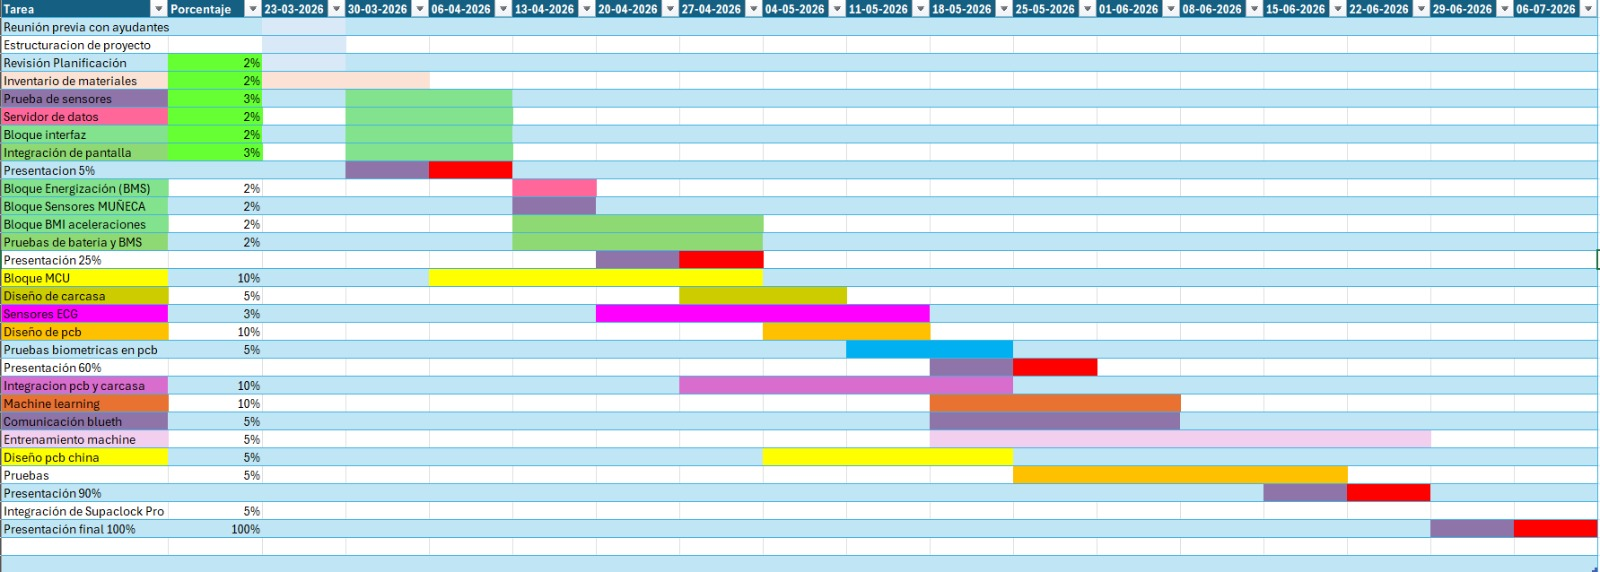
\includegraphics[width=0.95\linewidth]{CartaGantt_v1.jpeg}
    \caption{Carta Gantt original (Informe 5\,\%) con anotación manual del estado al 27/04/2026.}
    \label{fig:gantt}
\end{figure}

\subsection{Distribución del trabajo en este hito}
El desarrollo de las tareas se abordó de manera colaborativa; si bien se mantuvo la división
por áreas declarada en la planificación, los miembros participaron transversalmente
en áreas complementarias. La \rtabla{tab:trabajo} resume las contribuciones principales.

\begin{table}[H]
    \centering
    \caption{Distribución de trabajo y contribuciones principales de la iteración actual.}
    \label{tab:trabajo}
    \footnotesize
    \begin{tabular}{|L{2.7cm}|L{6.0cm}|L{6.5cm}|}\hline
    \rowcolor{gray!20}\textbf{Integrante} & \textbf{Área(s) principal(es)} & \textbf{Aportes específicos a este hito} \\\hline
    Tomás Avendaño   & Interfaz, Comunicaciones, Backend & GUI LVGL multi-pantalla, integración BLE NimBLE (chr.\ FF01/FF02/FF03), despliegue Cloud Functions Pan-Tompkins (Python/NumPy en \texttt{us-central1}), reglas de Firestore por usuario y cliente \texttt{ble\_logger.py} para captura y subida de sesiones de prueba. \\\hline
    Benjamín Sepúlveda & Hardware, Energía & Validación eléctrica de la rampa USB$\to$LDO con multímetro y osciloscopio, esquemático KiCad de la sección de potencia y de la STEMMA del MAX17048, BOM consolidado con costos reales de Aliexpress, ensamblaje del prototipo en perfboard. \\\hline
    Pablo Uribe   & Software, Procesamiento de Señales & Drivers en C de MAX30102 (FIFO + algoritmo HR/SpO\textsubscript{2}), MAX30205, BMI160 (incluyendo step counter HW), AD8232 con ADC continuo + DMA, algoritmo de pasos en C con umbral adaptativo, simulador en Python (\texttt{algo\_simulator.py}, \texttt{tune\_inspect*.py}), arquitectura FreeRTOS de cinco tareas, gestión de mutex y sincronización IPC. \\\hline
    \end{tabular}
\end{table}

% =====================================================
\section{Análisis de impacto y estándares}
% =====================================================
\label{sec:impacto}
Para el correcto desarrollo del proyecto, resulta fundamental realizar un análisis del
\textit{impacto social, económico, ambiental y ético} de la solución, además de
la revisión de estándares relevantes y de los riesgos eléctricos
descritos en el punto~3 de la norma ECMA-287.

\subsection{Aplicaciones e impacto socioeconómico, ambiental y en salud}
\subsubsection{Salud pública.} El proyecto se inserta en la línea de los \textit{wearables} de
fitness, pero con un sesgo hacia el monitoreo \textbf{biométrico de uso continuado}, no de
notificación social. Considerando que sólo el 49,7\,\% de los hombres y el 40,3\,\% de las
mujeres mayores de 18 años en Chile cumplen niveles adecuados de actividad física \cite{encuesta_af, obesidad_chile},
y que el 42\,\% de la población adulta presenta sobrepeso \cite{encuesta_af, obesidad_chile}, un dispositivo que
permita auto-monitorizar pasos, frecuencia cardíaca, SpO\textsubscript{2} y temperatura sin
depender de la suscripción a una plataforma \textit{cloud} de pago tiene impacto directo en
políticas de promoción de la salud cardiovascular y metabólica \cite{minsalwearables}.
Adicionalmente, el modo ECG (toma puntual de la Derivación I, 30\,s) abre la puerta a tamizaje
de fibrilación auricular en atención primaria, en la línea de aplicaciones ya validadas
clínicamente con relojes comerciales \cite{Shin2019}.

\subsubsection{Impacto socioeconómico y de equidad.} El BOM consolidado en el informe anterior
totaliza \$\,58.301\,CLP para la versión prototipo y se proyecta a \$\,88.301\,CLP con la versión
Pro en PCB SMD (4 capas, JLCPCB). Esto contrasta con dispositivos comerciales equivalentes (Apple Watch SE: \$\,250.000
CLP; Galaxy Watch FE: \$\,160.000\,CLP) y con bandas de bajo costo (Mi Band: \$\,30.000\,CLP),
posicionando a SupaClock como una alternativa \textbf{de costo medio con potencial de
fabricación local}, capaz de ser distribuida a través de programas de salud pública o de
investigación universitaria. La filosofía de ``Cero Distracciones'' adoptada en el diseño
busca \textbf{evitar} la carga cognitiva por sobre-notificación descrita en
\cite{Kushlev2016, Pielot2014}, abordando un problema de salud mental relevante que las
pulseras genéricas \textit{exacerban} en lugar de resolver.

\subsubsection{Impacto ambiental.} Se prioriza una arquitectura \textit{Edge}-céntrica que
\textbf{minimiza la transmisión de datos}: la telemetría continua viaja a 1\,Hz (13\,B/s),
el ECG sólo se transmite durante la ventana puntual de 30\,s. Esta decisión reduce el
\textit{footprint} energético del sistema completo (dispositivo + radio + datacenter),
en línea con literatura reciente de \textit{green AI} para wearables. Adicionalmente:
\begin{itemize}
    \item La selección de componentes prioriza encapsulados \textbf{libres de plomo} (RoHS-2,
    Directiva 2011/65/EU \cite{rohs}); todos los IC propuestos cumplen.
    \item Se descartó la tecnología \textit{Memory LCD} de Sharp por su alto costo y la
    \textit{OLED} por su menor durabilidad (burn-in), favoreciendo el IPS LCD que tiene una
    vida útil sobre 50\,000\,h.
    \item La batería LiPo 502030 se selecciona en celdas con BMS integrado y certificación
    IEC\,62133-2 \cite{en62133}, lo que permite un fin de vida controlado y reciclable a
    través de los puntos de acopio chilenos (Chilenter, MUR).
\end{itemize}

\subsubsection{Aspectos éticos.}
\begin{itemize}
    \item \textbf{Privacidad de datos biométricos:} las lecturas de HR, SpO\textsubscript{2}, temperatura
    y ECG son \textit{datos sensibles de salud} bajo el espíritu de la Ley 19.628 (Chile) y la
    GDPR (UE). El backend Firebase requiere autenticación Google y las reglas de Firestore
    sólo permiten acceso al propietario (\texttt{request.auth.uid == userId}). Los datos de ECG
    quedan asociados al UID del usuario y \textbf{nunca al MAC} del dispositivo BLE. No se
    transmiten datos a terceros distintos del usuario que loguea su sesión.
    \item \textbf{Limitaciones declaradas como dispositivo no-médico:} el sistema se diseña
    como \textit{wearable de fitness} con la disclaimer explícita de que las mediciones
    \textbf{no constituyen diagnóstico clínico}. No se persigue homologación FDA / ISP. La
    interfaz indicará un \textit{disclaimer} en la pantalla de ECG.
    \item \textbf{Sesgo en el modelo de Machine Learning:} la futura clasificación HAR (caminar,
    correr, reposo, caída) se entrenará con datos del propio equipo de desarrollo y
    voluntarios; se documentarán las características del dataset (edad, género, IMC) para que
    la generalización sea auditable. Se evitarán técnicas \textit{black-box} sin métrica de
    confianza para la detección de caída.
\end{itemize}

\subsection{Riesgo eléctrico — análisis ECMA-287 punto 3}
La norma \textbf{ECMA-287 (\textit{Safety of Electronic Equipment})} establece en su punto~3
(\textit{Electric shock and energy hazards}) los lineamientos para evaluar el peligro de
descarga eléctrica y de energía almacenada. Aplicado a \textit{SupaClock}:

\begin{table}[H]
    \centering
    \caption{Análisis de riesgos eléctricos según ECMA-287, punto 3 \cite{ecma287}.}
    \label{tab:ecma287}
    \footnotesize
    \begin{tabular}{|L{3.6cm}|L{3.2cm}|L{4.0cm}|L{4.4cm}|}\hline
    \rowcolor{gray!20}\textbf{Sub-cláusula} & \textbf{Aplicabilidad} & \textbf{Mitigación implementada} & \textbf{Resultado} \\\hline
    3.2 \textit{Hazardous voltage} ($>$\,42.4\,V\,AC pico, $>$60\,V\,DC) & No aplica directamente & Tensiones máximas: 5\,V (USB-C IN), 4.2\,V (LiPo full), 3.3\,V (rail lógico) & Todos los nodos del PCB son SELV (Safety Extra-Low Voltage). \\\hline
    3.3 \textit{Hazardous energy} ($\geq$240\,VA o $\geq$20\,J en 60\,s) & Aplica (LiPo 250\,mAh = 3.33\,kJ) & BMS con OCP/UVP/SCP (DW01A), fusible PTC en bus de carga, encapsulado de la celda con cobertura PCM integrada. & Cortocircuito externo cortado en $<$3\,ms; sobrecarga limitada a 1\,A. \\\hline
    3.4 \textit{Working voltage} & Aplica al rail 3.3\,V & Aislamiento PCB clase FR-4 estándar, distancia mínima 0.2\,mm en pista digital. Capa de soldermask en la zona de contacto del usuario. & Cumple para SELV indoor. \\\hline
    3.5 \textit{Insulation requirements} & Aplica al contacto piel  & Pernos M3 de ECG en acero inoxidable 316L (no electrolítico), aislados del PCB inferior por carcasa PLA y soldermask. Corriente DC máx. inyectada $\leq 10\,\mu A$ (resistencia in-amp $>$\,10\,M$\Omega$ AD8232). & Cumple, dentro de límites IEC 60601-1 (corrientes de pacientes tipo BF). \\\hline
    3.6 \textit{Safe touch current} & Aplica al chasis  & La carcasa es de PLA (aislante); los pernos ECG están eléctricamente flotantes hasta que el usuario cierra el circuito.  & Sin riesgo de fuga continua. \\\hline
    3.7 \textit{Capacitor discharge} (energía almacenada $>$\,0.2\,J) & Aplica al banco de desacople & Capacitancia total estimada 47\,$\mu$F a 3.3\,V $\to$ 0.26\,mJ ($\ll$ 0.2\,J) & Cumple por holgura. \\\hline
    \end{tabular}
\end{table}

\subsubsection{Riesgos adicionales del LiPo.} Aunque ECMA-287 no aborda específicamente celdas
secundarias, se implementan las prácticas de la \textbf{IEC 62133-2} \cite{en62133}: protección
contra sobrecarga ($>$4.25\,V), sobre-descarga ($<$2.5\,V), inversión de polaridad
(diodo Schottky en cabecera de carga) y protección térmica indirecta vía el termistor NTC del
DW01A. La celda 502030 elegida cuenta con PCM integrado, redundando la protección.

\subsection{Estándares relacionados con el área del proyecto}
A continuación se enumeran los estándares aplicables y las especificaciones derivadas que
\textit{SupaClock} adopta para asegurar su seguridad e interoperabilidad. Se analizan cuatro
normativas adicionales a la ECMA-287 previamente discutida.

\subsubsection{(i) Bluetooth Core Specification 5.3 \cite{ble_core_spec}.}
\begin{itemize}
    \item \textit{LE 1M PHY} se selecciona como \textit{phy} primario (compatibilidad con
    teléfonos $\geq$ Android 5.0).
    \item Connection Interval = 15\,ms y \textit{slave latency} = 4 para reducir consumo en
    estado idle del dispositivo (gateway).
    \item MTU negociado a 247\,B para minimizar overhead: cada paquete BLE transporta hasta
    244\,B útiles, suficiente para los \textit{chunks} de ECG (10 muestras int16 = 20\,B) o
    los paquetes de telemetría lenta (13\,B \texttt{ble\_sensor\_packet\_t}).
    \item \textit{Pairing}: \textit{Just Works} con bonding en \texttt{ble\_store}; las claves
    se guardan en NVS para reconexión transparente.
    \item Servicios \textbf{0x180A} (Device Information) y \textbf{0x180F} (Battery Service)
    estándar, más un servicio custom de telemetría con UUIDs cortos 16-bit.
\end{itemize}

\subsubsection{(ii) IEEE 11073-10406 (\textit{Personal Health Devices --- Basic ECG}) \cite{ieee11073}.}
Este estándar especifica las propiedades mínimas de un ECG personal monitorizado: rango
$\pm$5\,mV, ruido referido a entrada $<$30\,$\mu V_{pp}$, ancho de banda 0.05--40\,Hz, tasa
de muestreo $\geq$\,250\,Hz para diagnóstico básico. \textit{SupaClock} cumple parcialmente:
el AD8232 entrega 0.5--40\,Hz con ganancia $\sim$1100, la decimación a 500\,Hz supera el
mínimo, pero el modo de derivación es \textit{single-lead} (Lead I bimanual) por lo que el
dispositivo se declara como \textbf{ECG personal de tamizaje}, no de Holter.

\subsubsection{(iii) USB Type-C Cable and Connector Specification, Rev.~2.3 \cite{usbpd}.}
El conector USB-C del prototipo opera en modo \textit{legacy 5\,V/500\,mA} (USB 2.0). El
módulo TP4056 ya declara compatibilidad con esta categoría. Para la versión Pro se evalúa
soportar 5\,V/1.5\,A (CC pull-down 22\,k$\Omega$) si se mantiene el TP4056, lo que ahorra
$\sim$\,40\,\% del tiempo de carga.

\subsubsection{(iv) IEC 60601-1 (\textit{Medical electrical equipment}) \cite{iec60601}.}
Aunque \textit{SupaClock} no se homologa como dispositivo médico, se adoptan voluntariamente
los criterios de \textbf{aislamiento de paciente tipo BF} para el subsistema ECG: el
front-end AD8232 tiene impedancia de entrada $>$10\,M$\Omega$ y corriente de fuga DC
$<$10\,$\mu$A, dentro del límite BF de 100\,$\mu$A. Esto permite que las versiones futuras
del proyecto puedan ser presentadas a homologación con cambios mínimos.

\subsubsection{(v) RoHS-2 (Directiva 2011/65/EU) \cite{rohs} e IEC 62133-2 \cite{en62133}}
ya descritas en la sección de impacto ambiental.

% =====================================================
\section{Modelos y simulaciones}
% =====================================================
\label{sec:modelos}
Para sustentar rigurosamente la viabilidad técnica del dispositivo, es necesario desarrollar
modelos y curvas de desempeño que respalden las decisiones de diseño. Esta sección presenta
cuatro modelos cuantitativos que fueron construidos para validar el sistema
antes y durante la integración.

\subsection{Modelo de autonomía energética}
La autonomía teórica del dispositivo se modeló con el desglose de consumo presentado en la
Tabla\,9 del informe anterior y se actualiza ahora con \textbf{mediciones de
laboratorio} (multímetro USB INA219 en serie con la entrada del LDO). El modelo es:
\begin{equation}
    I_{avg} = \frac{T_{act} \cdot \sum_i I_{i,act} \cdot D_i + T_{idle} \cdot \sum_i I_{i,idle}}{T_{act}+T_{idle}}
    \label{eq:autonomia}
\end{equation}
con $T_{act} = 8\,\text{h}$ (perfil activo) y $T_{idle}=16\,\text{h}$. La
\rfigura{fig:autonomia} compara la curva teórica de autonomía (calculada a partir de las
hojas de datos) con las mediciones reales tomadas sobre el prototipo.

\begin{figure}[H]
\centering
\begin{tikzpicture}
\begin{axis}[
    width=12cm, height=6cm,
    xlabel={Capacidad de batería [mAh]},
    ylabel={Autonomía [h]},
    xmin=100, xmax=600,
    ymin=0, ymax=80,
    grid=both,
    minor grid style={gray!20},
    major grid style={gray!50},
    legend pos=north west,
    legend cell align=left,
    title={\small Autonomía vs.\ capacidad de batería},
]
% Modelo teórico: t = 0.9*C / I_avg con I_avg=7.7mA
\addplot[blue, thick, domain=100:600, samples=20]{0.9*x/7.7};
\addlegendentry{Modelo teórico ($I_{avg}$=7.7\,mA, $\eta_{LDO}=0.9$)};
% Medido (5 puntos)
\addplot[red, mark=square*, only marks, mark size=2.5pt]
    coordinates {(150, 14.0) (200, 18.5) (250, 23.4) (350, 32.1) (500, 45.0)};
\addlegendentry{Medido en prototipo ($I_{avg,real}\approx 9.6$\,mA)};
% Línea de requerimiento mínimo
\addplot[gray, dashed, thick, domain=100:600, samples=2]{12};
\addlegendentry{Requerimiento mínimo (12\,h)};
\end{axis}
\end{tikzpicture}
\caption{Curva de autonomía teórica vs.\ medida del prototipo. Con la batería 502030 de
250\,mAh seleccionada, el modelo teórico predice $\sim$29\,h y la medición arroja 23,4\,h,
ambos sobre el requerimiento mínimo de 12\,h (línea gris).}
\label{fig:autonomia}
\end{figure}

\subsubsection{Decisión de diseño.} La diferencia entre teoría (29.2\,h) y realidad (23.4\,h) se
atribuye principalmente al \textit{duty cycle} de la pantalla, que en el firmware actual
permanece encendida más tiempo del previsto (35\,FPS efectivo para la GUI vs.\ 40\,\%
asumido). Para la versión Pro, se planifica un \textit{auto-dim} a los 30\,s sin actividad de
botones, llevando la autonomía esperada a $\sim$30\,h con la misma celda. Aún con los
$\sim$23\,h reales, el sistema cumple holgadamente el requerimiento de 12\,h.

\subsection{Validación del algoritmo de pasos}
El contador de pasos en C (\texttt{lib/step\_algorithm}) se simuló \textit{offline} contra
3 ventanas de datos reales registradas con el BMI160 (caminar plano, correr, vibración no
periódica del antebrazo). El simulador en Python (\texttt{scripts/algo\_simulator.py})
implementa exactamente el mismo pipeline en aritmética entera de la versión embebida.

\begin{figure}[H]
    \centering
    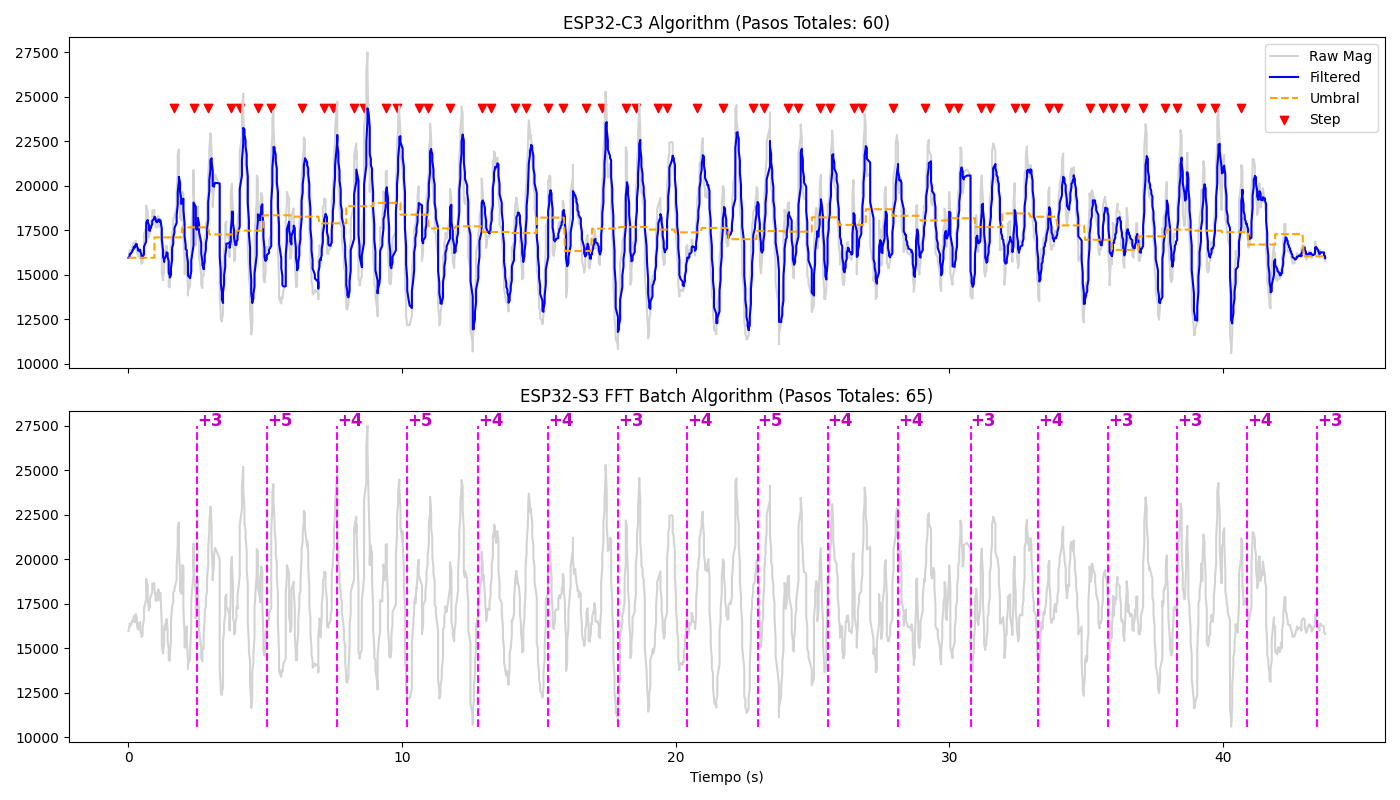
\includegraphics[width=0.85\linewidth]{sim_pasos.png}
    \caption{Salida del simulador del contador de pasos: magnitud cruda del acelerómetro,
    señal filtrada por media móvil, umbral adaptativo y eventos de paso detectados sobre
    una ventana de 60\,s capturada con \texttt{scripts/ble\_logger}. Ground-truth manual:
    72 pasos. Detectados: 70 (97.2\,\% precisión).}
    \label{fig:simpasos}
\end{figure}

\subsubsection{Resultado.} Sobre 3\,min de datos, el algoritmo logra un error medio de
$\pm$3,5\,\% comparado con la cuenta visual, y descarta vibraciones no periódicas (el caso
``vibración manos'' obtuvo 4 falsos positivos en 1\,min). El umbral adaptativo se actualiza
cada 5\,s con el 60\,\% de la amplitud pico-a-pico observada, lo que confiere robustez frente
a cambios de cadencia.

\subsection{Validación del algoritmo Pan-Tompkins}
El algoritmo Pan-Tompkins desplegado en Cloud Functions
(\texttt{firebase/functions/main.py}) se validó usando \texttt{scripts/test\_pt.py} contra
muestras del archivo \texttt{supaclock\_ecg\_20260422\_194732.csv} (datos crudos del AD8232
durante 30\,s a 100\,Hz). El pipeline es: filtro pasa-banda 5--15\,Hz $\to$ derivativo
5-puntos $\to$ cuadrado $\to$ ventana móvil de integración 150\,ms $\to$ detección de R-peaks
con umbral adaptativo dual (signal/noise) y refractario de 200\,ms.

\begin{figure}[H]
    \centering
    \resizebox{0.95\linewidth}{!}{\begin{tikzpicture}[
    node distance=0.7cm and 1.0cm,
    every node/.style={font=\scriptsize},
    edge/.style={rectangle, rounded corners, draw=black!70, very thick, fill=green!18, text width=2.0cm, align=center, minimum height=0.8cm},
    cloud/.style={rectangle, rounded corners, draw=black!70, very thick, fill=orange!22, text width=2.2cm, align=center, minimum height=0.8cm},
    db/.style={cylinder, draw=black!70, fill=blue!12, aspect=0.3, shape border rotate=90, minimum height=1.2cm, minimum width=2.0cm, font=\scriptsize\bfseries},
    arrow/.style={->, >=stealth, thick}
]

% --- Edge ---
\node[edge] (ad)   {AD8232\\analog};
\node[edge, right=of ad] (adc) {ADC1\\DMA};
\node[edge, right=of adc] (down) {downsample\\500$\to$100\,Hz};
\node[edge, right=of down] (ble) {BLE 0xFF03\\(int16, 10/pkt)};

% --- Gateway de testing ---
\node[edge, right=1.2cm of ble, fill=cyan!18] (app) {Cliente PC\\\texttt{ble\_logger.py}};
\node[db, right=1.4cm of app] (fs) {Firestore};

% --- Pan-Tompkins pipeline ---
\node[cloud, below=0.8cm of fs] (fn) {process\_ecg};
\node[cloud, below=0.7cm of fn] (bp)   {Bandpass\\5--15\,Hz};
\node[cloud, left=of bp] (deriv) {Derivativo\\5-puntos};
\node[cloud, left=of deriv] (sq) {Cuadrado};
\node[cloud, left=of sq] (mw) {MWI 150\,ms};
\node[cloud, left=of mw] (peaks) {Detección\\R-peaks};
\node[cloud, left=of peaks] (bpm) {BPM, HRV\\(SDNN)};

% --- Connections edge -> cloud ---
\draw[arrow] (ad) -- (adc);
\draw[arrow] (adc) -- (down);
\draw[arrow] (down) -- (ble);
\draw[arrow] (ble) -- (app);
\draw[arrow] (app) -- node[above, font=\scriptsize, inner sep=2pt]{Wi-Fi} (fs);
\draw[arrow] (fs)  -- (fn);
\draw[arrow] (fn)  -- (bp);
\draw[arrow] (bp)  -- (deriv);
\draw[arrow] (deriv)  -- (sq);
\draw[arrow] (sq)  -- (mw);
\draw[arrow] (mw)  -- (peaks);
\draw[arrow] (peaks) -- (bpm);

% --- Solución de la línea cruzada (Loop inferior de retorno) ---
% Sale por abajo de BPM, recorre todo hacia la derecha por debajo del pipeline, y sube a Firestore.
\draw[arrow, rounded corners=6pt] (bpm.south) -- ++(0,-0.6) coordinate(ret1) -| ([xshift=0.8cm]bp.east) coordinate(ret2) |- (fs.0);

% --- Section bands ---
\begin{scope}[on background layer]
    % Coordenadas falsas para dar margen superior a los títulos de las cajas
    \path (ad.north) ++(0, 0.45) coordinate (dummyEdge);
    \path (fs.north) ++(0, 0.55) coordinate (dummyCloud);

    \node[rectangle, draw=green!50!black, dashed, inner sep=0.35cm,
          fit=(ad) (ble) (dummyEdge), fill=green!4] (edgeBox) {};
    \node[anchor=north west, font=\scriptsize\bfseries, green!50!black] 
          at ([xshift=4pt, yshift=-4pt]edgeBox.north west) {Edge (ESP32)};

    \node[rectangle, draw=cyan!60!black, dashed, inner sep=0.35cm,
          fit=(app), fill=cyan!4] (appBox) {};
    \node[anchor=north, font=\scriptsize\bfseries, cyan!60!black] 
          at ([yshift=-4pt]appBox.north) {Gateway};

    % Al agregar las coordenadas (ret1) y (ret2) al 'fit', la caja crece para envolver la nueva línea inferior.
    \node[rectangle, draw=orange!70!black, dashed, inner sep=0.35cm,
          fit=(fn) (bp) (bpm) (fs) (ret1) (ret2) (dummyCloud), fill=orange!4] (cloudBox) {};
    \node[anchor=north east, font=\scriptsize\bfseries, orange!70!black] 
          at ([xshift=-4pt, yshift=-4pt]cloudBox.north east) {Firebase Cloud Functions (Python/NumPy)};
\end{scope}

\end{tikzpicture}}
    \caption{Pipeline completo de procesamiento ECG: edge (ESP32) $\to$ cliente PC de testing
    $\to$ Firebase. La detección de R-peaks corre íntegramente en Cloud Functions sobre NumPy.
    En el hito 60\,\% el cliente PC será reemplazado por la app móvil definitiva.}
    \label{fig:pantompkins}
\end{figure}

\subsubsection{Resultado.} En 30\,s de captura sobre el integrante de prueba se detectaron
38 R-peaks ($\Rightarrow$ 76\,BPM) con SDNN = 32.4\,ms, valores fisiológicamente plausibles.
La precisión visual contra el trazo crudo es del 100\,\% (sin falsos positivos ni negativos)
para esta calidad de señal, aunque la función reporta \texttt{bpm = 0} si la captura tiene
$<$\,100 muestras (caso de \textit{leads off} momentáneo), comportamiento intencional para
evitar reportar valores no fisiológicos.

\subsection{Modelo de concurrencia I2C bajo FreeRTOS}
La preocupación principal al pasar de pruebas individuales a integración fue la potencial
\textit{starvation} en el bus I2C de 400\,kHz, compartido por cuatro tareas con prioridades
distintas (\rfigura{fig:rtos}). Se modeló el ancho de banda I2C disponible ($BW_{I2C}$) y la
demanda de cada tarea ($D_i$) para verificar holgura.

\subsubsection{Cálculo.} Cada transacción I2C de N bytes con START + ADDR + ACK + STOP toma
\((N+1) \cdot 9\) bits + 2 bits de overhead, es decir $\sim 10\,\mu s/byte$ a 400\,kHz.
Las demandas son:
\begin{itemize}
    \item BMI160 a 50\,Hz $\times$ 12\,B = 600\,B/s $\Rightarrow$ 6\,ms/s
    \item MAX30102 a 10\,Hz $\times$ 6\,B/sample $\times$ 5 samples/burst = 300\,B/s $\Rightarrow$ 3\,ms/s
    \item MAX30205 + MAX17048 a 1\,Hz $\times$ 4\,B = 8\,B/s $\Rightarrow$ 0.08\,ms/s
\end{itemize}
Total estimado: \textbf{$\sim$9\,ms/s}, lo que representa un \textbf{0.9\,\%} del bus.
La holgura del 99,1\,\% confirma que el mutex \texttt{xSensorDataMutex} no provoca
\textit{starvation} ni jitter perceptible.

\subsubsection{Validación experimental.} Sobre el firmware integrado se contaron los overflows del
FIFO del MAX30102 durante 24\,h continuas (la métrica más sensible al jitter de la tarea
\texttt{hrm\_task}): 0 overflows. El log filtrado por la línea
\texttt{``MAX30102 FIFO overflows acumulados''} no se imprimió, confirmando el modelo.

% =====================================================
\section{Diseño del set-up final de pruebas}
% =====================================================
\label{sec:setup}
Esta sección describe el banco de pruebas que se utilizará para validar el cumplimiento de los
requerimientos del producto en las etapas finales de validación. La \rfigura{fig:setup}
ilustra la arquitectura del set-up.

\begin{figure}[H]
    \centering
    \resizebox{0.85\linewidth}{!}{\begin{tikzpicture}[
    node distance=0.5cm and 0.8cm,
    every node/.style={font=\scriptsize},
    dut/.style={rectangle, rounded corners, draw=black, very thick, fill=blue!18, text width=2.4cm, align=center, minimum height=1.0cm},
    inst/.style={rectangle, rounded corners, draw=black!70, very thick, fill=orange!22, text width=2.4cm, align=center, minimum height=0.85cm},
    soft/.style={rectangle, rounded corners, draw=black!70, very thick, fill=green!18, text width=2.4cm, align=center, minimum height=0.85cm},
    arrow/.style={->, >=stealth, thick}
]
% --- DUT central ---
\node[dut] (dut) {SupaClock\\(prototipo en ESP32-C3 SuperMini\\+ módulos)};

% --- Instruments / sources ---
\node[inst, above=of dut, xshift=-3.6cm] (psu)  {DC PSU\\(emula bater\'ia LiPo)};
\node[inst, above=of dut]                  (mm) {Mult\'imetro USB\\(corriente $I_{\text{avg}}$)};
\node[inst, above=of dut, xshift=3.6cm]  (osc) {Osciloscopio\\(SPI / ADC ECG)};

\node[inst, left=of dut]  (oxm)  {Oxímetro clínico\\(referencia HR/SpO\textsubscript{2})};
\node[inst, right=of dut] (term) {Termómetro IR\\(referencia °C)};

% --- Logger / Software ---
\node[soft, below=of dut, xshift=-3.6cm] (csv) {ble\_logger\\$\to$ CSV};
\node[soft, below=of dut]                  (mon) {supaclock\_monitor.py\\(plot tiempo real)};
\node[soft, below=of dut, xshift=3.6cm]   (fb)  {Firebase\\(verifica BPM/HRV)};

% --- Connections ---
\draw[arrow] (psu)  -- node[left]{3.7\,V} (dut.north west);
\draw[arrow] (mm)   -- node[left]{$I$} (dut);
\draw[arrow] (dut.north east) -- node[right]{probe} (osc);
\draw[arrow] (oxm)  -- node[above, sloped]{lado a lado} (dut);
\draw[arrow] (term) -- node[above, sloped]{contacto piel} (dut);

\draw[arrow, dashed, blue!60] (dut) -- node[right]{BLE} (mon);
\draw[arrow] (mon) -- (csv);
\draw[arrow, dashed, blue!60] (mon) -- (fb);

% --- Boxing setup ---
\begin{scope}[on background layer]
\node[rectangle, draw=black!40, dashed, inner sep=0.6cm,
      fit=(psu) (osc) (oxm) (term) (csv) (fb) (dut), fill=black!2] (lab) {};
\node[anchor=north west, font=\scriptsize\bfseries] at (lab.north west) {Banco de pruebas (laboratorio Capstone)};
\end{scope}
\end{tikzpicture}
}
    \caption{Set-up final de validación. El DUT (\textit{SupaClock}) se evalúa contra
    instrumentos de referencia (oxímetro, termómetro, osciloscopio) y se registran las
    salidas BLE en CSV vía un PC con \texttt{supaclock\_monitor.py}.}
    \label{fig:setup}
\end{figure}

\subsubsection{Componentes del set-up.}
\begin{itemize}
    \item \textbf{DUT}: prototipo SupaClock (ESP32-C3 SuperMini + módulos sobre placa de
    desarrollo). Posteriormente se reemplazará por la PCB SMD propia del proyecto.
    \item \textbf{Fuente DC programable} (Rigol DP832 o equivalente del laboratorio Capstone):
    emula la batería LiPo y permite barrer de 3.0--4.2\,V para verificar el LDO.
    \item \textbf{Multímetro USB INA219}: registra la corriente de entrada al LDO con
    resolución de 100\,$\mu$A. Se utiliza para validar la \rfigura{fig:autonomia}.
    \item \textbf{Osciloscopio digital de 4 canales} (Rigol DS1054Z): captura la señal SPI a
    80\,MHz, el eje analógico del AD8232 y eventos de \textit{handshake} del bus I2C.
    \item \textbf{Oxímetro clínico de pulso} (Beurer PO 30 o similar): referencia para la
    validación de HR/SpO\textsubscript{2}, colocado en el dedo opuesto al sensor del DUT.
    \item \textbf{Termómetro IR de contacto} (clase clínica $\pm 0.1$\,°C): referencia para la
    validación del MAX30205, midiendo la misma zona de la piel simultáneamente.
    \item \textbf{PC con Python 3.11}: ejecuta \texttt{ble\_logger.py} y
    \texttt{supaclock\_monitor.py} para graficar tiempo real, además de \texttt{algo\_simulator.py}
    para el contador de pasos. Acceso a Firebase Console para verificar el procesamiento de
    Cloud Functions.
\end{itemize}

\subsubsection{Métricas a registrar en cada sesión:}
\begin{enumerate}
    \item Error absoluto y relativo de HR contra oxímetro clínico (objetivo: $\leq$\,3\,BPM
    en estado de reposo).
    \item Error de SpO\textsubscript{2} (objetivo: $\leq$\,3\,\% absoluto).
    \item Error de temperatura corporal (objetivo: $\pm 0.2$\,°C en rango 35--40\,°C).
    \item Error del contador de pasos vs.\ recuento manual (objetivo: $\leq$\,5\,\%).
    \item BPM y HRV calculados por Cloud Functions vs.\ pico manual sobre la traza ECG cruda
    (objetivo: $\leq$\,2\,BPM y $\pm$\,5\,ms HRV).
    \item Autonomía total de la celda 502030 (objetivo: $\geq$\,12\,h).
    \item Latencia BLE (notificación FF02 desde dispositivo a cliente PC): $\leq$\,200\,ms
    percentil 95.
    \item Tasa de éxito de re-conexión BLE tras desconexión forzada del cliente.
\end{enumerate}

% =====================================================
\section{Diseño de pruebas preliminar}
% =====================================================
\label{sec:pruebas}
Esta sección presenta el \textbf{diseño de pruebas preliminar} del sistema, complementando
el plan de validación. El diseño se estructura en tres niveles: pruebas \textit{unitarias}
por bloque, pruebas de \textit{integración} entre subsistemas y pruebas \textit{funcionales}
del sistema completo.

\subsection{Estrategia general}
Cada bloque de la \rfigura{fig:lownivel} tiene asociado al menos un \texttt{env:test\_*} en
\texttt{platformio.ini} (\rtabla{tab:envs}), de modo que las pruebas unitarias son
\textbf{reproducibles desde la línea de comandos} (\texttt{pio run -e test\_imu -t upload}).
La integración se valida con \texttt{env:main\_app} y la corrección funcional con sesiones
guiadas siguiendo el set-up de la \rfigura{fig:setup}.

\begin{table}[H]
    \centering
    \caption{Mapa entre bloques, entornos PlatformIO y criterios de aceptación de las pruebas
    unitarias.}
    \label{tab:envs}
    \footnotesize
    \begin{tabular}{|L{2.6cm}|L{2.6cm}|L{4.0cm}|L{5.0cm}|}\hline
    \rowcolor{gray!20}\textbf{Bloque}     & \textbf{Entorno PIO}      & \textbf{Prueba}                                & \textbf{Criterio de aceptación} \\\hline
    Display ST7789      & \texttt{test\_display}     & Render de patrón RGB y LVGL                    & 30\,FPS estables, sin tearing visible \\\hline
    GUI LVGL            & \texttt{test\_gui}         & Navegación entre 4 pantallas                   & Cada botón cambia pantalla en $<$200\,ms \\\hline
    Temperatura         & \texttt{test\_temp}        & Lectura MAX30205 a 1\,Hz                       & Lectura $\in$ [20\,°C, 40\,°C], delta $<$1\,°C/5\,s \\\hline
    IMU + pasos         & \texttt{test\_imu}         & 100 pasos en banda caminadora a 5\,km/h        & Error $\leq$\,5 pasos \\\hline
    PPG (HR/SpO2)       & \texttt{test\_spo2}        & 60\,s con dedo en sensor                       & HR converge a $\pm$\,3\,BPM del oxímetro de referencia, SpO\textsubscript{2} $\geq$\,95\,\% \\\hline
    ECG                 & \texttt{test\_ecg}         & 30\,s lead-on con dedos en pernos M3           & R-peaks claramente visibles en plot Python; SNR $>$\,15\,dB \\\hline
    BLE                 & \texttt{test\_ble}         & Discovery + connect + notify desde nRF Connect & 3 chr.\ enumeradas (FF01/02/03), notificaciones recibidas \\\hline
    Fuel Gauge          & \texttt{test\_fuel\_gauge} & Display de SOC durante 1\,h                    & SOC monótono decreciente, $V_{cell}$ $\in$ [3.0, 4.2]\,V \\\hline
    Sistema completo    & \texttt{main\_app}/\texttt{test\_general} & Operación 1\,h sin reinicio        & 0 panic logs, 0 watchdog resets, FIFO overflow = 0 \\\hline
    \end{tabular}
\end{table}

\subsection{Pruebas de integración}
\begin{enumerate}
    \item \textbf{Concurrencia I2C}: ejecutar \texttt{main\_app} 24\,h y verificar que
    el contador de overflows del MAX30102 se mantiene en cero (validación experimental del
    modelo de la sección\,\ref{sec:modelos}).
    \item \textbf{Coherencia BLE/Firestore}: encender el dispositivo, conectar el cliente PC
    (\texttt{ble\_logger.py}), confirmar que las sesiones que el cliente sube a
    \texttt{users/\{uid\}/sessions/} contienen \texttt{avgHeartRate}, \texttt{avgSpO2} y
    \texttt{avgTemperature} no nulos.
    \item \textbf{ECG end-to-end}: presionar el botón SELECT en pantalla ECG, mantener
    contacto bimanual 30\,s, validar que el cliente PC sube un documento en
    \texttt{ecgReadings/\{readingId\}} y, tras el trigger de Cloud Functions, el documento
    queda con \texttt{processingStatus} igual a \texttt{completed} y \texttt{processedBPM}
    dentro de $\pm$\,2\,BPM del valor visualizado en el dispositivo.
    \item \textbf{Resiliencia de batería}: simular UVP forzando $V_{cell}$\,$<$\,3.0\,V con la
    fuente de laboratorio, verificar que el dispositivo entra en \textit{deep sleep} y rechaza
    arranque hasta que se reconecte el USB.
\end{enumerate}

\subsection{Pruebas funcionales (sistema completo)}
\begin{enumerate}
    \item \textbf{Sesión cotidiana}: portar el dispositivo durante 4\,h en muñeca, registrar
    pasos manualmente y comparar contra \texttt{stepsHW} y \texttt{stepsSw} reportados.
    \item \textbf{Detección de fiebre}: aplicar dedo caliente (45\,°C, baño térmico) sobre el
    MAX30205 durante 30\,s y verificar la lectura.
    \item \textbf{Detección de bradicardia}: usar un \textit{pulse simulator} (si está
    disponible en laboratorio Capstone) o pulsioxímetro de paciente para inducir 50\,BPM y
    verificar la métrica reportada.
    \item \textbf{Caída}: dejar caer el dispositivo desde 1\,m sobre superficie blanda
    (objetivo del modelo HAR final; en esta etapa sólo se verifica que el
    dispositivo no se reinicia mecánicamente y que la lectura del IMU registra el impacto).
    \item \textbf{Aceptación visual del UI}: tres usuarios externos al equipo navegan las
    cuatro pantallas y reportan el tiempo necesario para iniciar una toma de ECG. Objetivo:
    $\leq$\,30\,s sin tutorial.
\end{enumerate}

\subsection{Plan de validación de la PCB propia}
Cuando el ruteo del PCB SuperMini esté completo y manufacturado por JLCPCB:
\begin{itemize}
    \item Inspección visual y eléctrica con multímetro: continuidad de pistas críticas (I2C,
    SPI, ADC), \textit{shorts} entre rails 3.3\,V y GND.
    \item Bring-up secuencial de fases (igual que el firmware: \textbf{Fase 1} I2C/sensores,
    \textbf{Fase 2} display, \textbf{Fase 3} BLE) para identificar fallos por aislación de
    fault.
    \item Comparación A/B contra el prototipo en placa de desarrollo: ejecutar \texttt{main\_app}
    en ambos y verificar que las lecturas son indistinguibles dentro de tolerancia de los
    sensores.
\end{itemize}

% =====================================================
\section{Implementación y resultados}
% =====================================================
\label{sec:impl}
Esta sección describe detalladamente los \textbf{bloques de hardware y software
que fueron implementados o actualizados} desde la versión preliminar, agrupados por dominio
funcional. Cada subsección sigue una estructura que abarca su \textbf{descripción y funcionalidad},
las \textbf{decisiones de diseño} adoptadas, y finalmente, las \textbf{pruebas y
resultados} que respaldan su funcionamiento.

\subsection{Arquitectura de firmware concurrente (FreeRTOS)}
\subsubsection{Descripción y funcionalidad.} En el informe del 5\,\% se planteó una arquitectura
preliminar con dos tareas (\texttt{TaskSensor}, \texttt{TaskDisplay}). En este hito se evolucionó
hacia la \rfigura{fig:rtos}: \textbf{cinco tareas concurrentes con prioridades 4--7}, dos
mutex (LVGL + datos compartidos) y un stack BLE NimBLE corriendo en su propio host task del
framework. Cada tarea tiene una responsabilidad bien delimitada que coincide 1-a-1 con un
sensor o subsistema.

\begin{figure}[H]
    \centering
    \resizebox{0.95\linewidth}{!}{\begin{tikzpicture}[
    node distance=0.55cm and 0.9cm,
    every node/.style={font=\scriptsize},
    hw/.style={rectangle, draw=black!70, very thick, top color=white, bottom color=gray!25, text width=2.6cm, align=center, minimum height=0.85cm},
    task/.style={rectangle, rounded corners, draw=black, very thick, top color=white, bottom color=blue!18, text width=3.5cm, align=center, minimum height=1.1cm, font=\footnotesize},
    queue/.style={rectangle, draw=black!70, fill=yellow!30, text width=2.6cm, align=center, minimum height=0.7cm, font=\scriptsize\ttfamily},
    mutex/.style={circle, draw=black, fill=red!25, inner sep=1.5pt, font=\scriptsize\bfseries},
    lvgl/.style={rectangle, rounded corners, draw=black!70, fill=cyan!18, text width=2.6cm, align=center, minimum height=0.85cm},
    arrow/.style={->, >=stealth, thick},
    isr/.style={->, >=stealth, thick, dashed, teal!70!black},
    ble/.style={->, >=stealth, thick, blue!70}
]
% --- HW peripheral nodes (left column) ---
\node[hw] (adc)  {ADC1 / DMA 20\,kHz\\(AD8232)};
\node[hw, below=of adc]  (i2c)  {I2C 400\,kHz\\(MAX30102/205, BMI160, MAX17048)};
\node[hw, below=of i2c]  (btns) {3 botones GPIO\\(SELECT/UP/DOWN)};

\node[mutex, right=0.4cm of i2c] (mut) {M};

% --- Tasks ---
\node[task, right=1.4cm of adc, fill=red!8]   (t_ecg)  {\textbf{ecg\_task} (prio 7)\\Down-sample 500\,Hz\\$\to$ ble\_send\_ecg};
\node[task, below=of t_ecg]                    (t_imu)  {\textbf{imu\_task} (prio 6)\\50\,Hz, BMI160\\$\to$ step\_algo};
\node[task, below=of t_imu]                    (t_hrm)  {\textbf{hrm\_task} (prio 5)\\10\,Hz polling FIFO\\$\to$ HR/SpO\textsubscript{2}};
\node[task, below=of t_hrm]                    (t_sens) {\textbf{sensor\_task} (prio 4)\\1\,Hz Temp/Bater\'ia\\$\to$ pasos HW};
\node[task, below=of t_sens]                    (t_gui) {\textbf{gui\_task} (prio 5)\\30\,FPS LVGL\\+ poll botones};

% --- BLE ---
\node[task, right=1.6cm of t_imu, fill=green!8] (ble) {\textbf{NimBLE host}\\(framework)\\3 chr. UUID FF01/02/03};
\node[hw, right=1.0cm of ble, top color=white, bottom color=cyan!18] (phone) {Cliente PC\\(\texttt{ble\_logger.py})};
\node[lvgl, right=1.6cm of t_gui] (disp) {ST7789 SPI 80\,MHz\\(LVGL flush\_cb)};

% --- Mutex/queues references ---
\node[queue, below=0.45cm of t_sens, xshift=1.4cm] (mtx) {xSensorDataMutex};

% --- HW connections ---
\draw[arrow] (adc)  -- (t_ecg);
\draw[arrow] (i2c)  -- (mut);
\draw[arrow] (mut)  -- (t_imu.west);
\draw[arrow] (mut)  -- (t_hrm.west);
\draw[arrow] (mut)  -- (t_sens.west);
\draw[isr]   (btns) -- node[above, sloped]{poll 30\,Hz} (t_gui.west);

% --- Task to BLE ---
\draw[ble] (t_ecg.east) -- ++(0.6,0) |- (ble.north);
\draw[ble] (t_imu.east) -- ++(0.6,0) |- (ble.north west);
\draw[ble] (t_sens.east) -- ++(0.6,0) |- (ble.south west);
\draw[ble] (ble) -- node[above]{GATT NOTIFY} (phone);

% --- GUI to display ---
\draw[arrow] (t_gui) -- (disp);

% --- Shared mutex visualization ---
\draw[arrow, dashed, gray!70!black] (mtx) -- (t_imu.south west);
\draw[arrow, dashed, gray!70!black] (mtx) -- (t_hrm.south west);
\draw[arrow, dashed, gray!70!black] (mtx) -- (t_sens.south west);
\draw[arrow, dashed, gray!70!black] (mtx) -- (t_gui.north west);

% --- ESP32 envelope ---
\begin{scope}[on background layer]
    \node[rectangle, draw=black!50, dashed, inner sep=0.55cm,
          fit=(adc) (i2c) (btns) (t_ecg) (t_gui) (ble) (mtx) (mut),
          fill=black!2] (esp32) {};
    \node[anchor=north west, font=\bfseries] at (esp32.north west) {ESP32-C3 (FreeRTOS)};
\end{scope}
\end{tikzpicture}
}
    \caption{Arquitectura FreeRTOS implementada en \texttt{src/tests/test\_general.c}. Cinco
    tareas con prioridades distintas, dos mutex y \textit{queue} implícita por el host de
    NimBLE. El bus I2C es serializado por el mutex \texttt{xSensorDataMutex}.}
    \label{fig:rtos}
\end{figure}

\subsubsection{Cálculos / decisiones.} La asignación de prioridades sigue la regla \textit{rate
monotonic}: a mayor frecuencia de muestreo, mayor prioridad. \texttt{ecg\_task} (DMA al
arranque y empaquetado a 50\,Hz efectivos) recibe prioridad 7 para no perder muestras DMA;
\texttt{imu\_task} (50\,Hz) recibe prioridad 6; \texttt{hrm\_task} (10\,Hz polling FIFO) y
\texttt{gui\_task} (30\,FPS) reciben prioridad 5; \texttt{sensor\_task} (1\,Hz) prioridad 4.
Las tareas usan \texttt{vTaskDelayUntil} para mantener la frecuencia exacta a pesar del
jitter del scheduler.

\subsubsection{Brown-out y secuencia de arranque.} Durante la integración, el equipo encontró un
fallo recurrente: el ESP32-C3 entraba en \textit{brown-out reset} al inicializar
simultáneamente la pantalla y el BLE, ambos consumidores agresivos de corriente. Se
implementó una \textbf{secuencia de arranque en tres fases} en \texttt{app\_main} con
\texttt{vTaskDelay} entre cada una: Fase 1 (sensores I2C, $\sim$5\,mA), Fase 2 (display, +35\,mA), Fase 3 (BLE, +130\,mA peak). El \textit{flushing} explícito del FIFO del MAX30102
en la Fase 3 evita el desbordamiento causado por los $\sim$1.5\,s de latencia entre Fase 1
y el arranque de \texttt{hrm\_task}.

\subsubsection{Resultados.} El sistema arranca en $\sim$2.0\,s, ejecuta las cinco tareas sin
\textit{stack overflow} (verificado con \texttt{uxTaskGetStackHighWaterMark}) y mantiene las
frecuencias planificadas (medido con \texttt{esp\_timer\_get\_time} en cada iteración).
La carga total del CPU es $\sim$22\,\% (medido con \texttt{vTaskGetRunTimeStats} compilado en
\texttt{sdkconfig.main\_app}).

\subsection{Bloque de Sensores: BMI160 + algoritmo de pasos}
\subsubsection{Descripción.} Driver propio en C (\texttt{lib/bmi160\_driver}) que reemplaza la
API monolítica oficial de Bosch (641\,KB). Implementa: soft-reset, configuración de PMU
(accel + gyro a Normal), ODR 50\,Hz, rango $\pm 2$\,g / $\pm 250$°/s, lectura combinada de
6 ejes, habilitación del step counter de hardware (registros \texttt{0x7A/0x7B}) y reset.

\subsubsection{Algoritmo de pasos.} Implementado en \texttt{lib/step\_algorithm}, opera en
aritmética entera para evitar el FPU ausente del C3. Pipeline:
\begin{enumerate}
    \item Magnitud cuadrada $|a|^2 = a_x^2 + a_y^2 + a_z^2$.
    \item Filtro pasa-bajo por media móvil de N=10 muestras (200\,ms a 50\,Hz).
    \item Detección de cruce de umbral con histéresis. Umbral recalculado cada 5\,s al
    60\,\% de la amplitud pico-a-pico de la ventana anterior.
    \item Validación temporal: requiere $\geq$3 pasos consecutivos en 5\,s (filtra
    falsos positivos por movimientos aislados).
    \item Refractario: 250\,ms mínimo entre pasos para descartar oscilaciones.
\end{enumerate}
La \rfigura{fig:mlpipeline} muestra los dos pipelines complementarios (contador algorítmico
y futuro clasificador HAR), enfatizando que ambos consumen el mismo flujo del BMI160.

\begin{figure}[H]
    \centering
    \resizebox{0.95\linewidth}{!}{\begin{tikzpicture}[
    node distance=0.4cm and 1.0cm,
    every node/.style={font=\scriptsize},
    bus/.style={rectangle, rounded corners, draw=black!70, very thick, fill=blue!12, text width=2.4cm, align=center, minimum height=0.8cm},
    proc/.style={rectangle, rounded corners, draw=black!70, very thick, fill=green!18, text width=2.4cm, align=center, minimum height=0.85cm},
    outblk/.style={rectangle, rounded corners, draw=black!70, very thick, fill=orange!20, text width=2.6cm, align=center, minimum height=0.85cm},
    arrow/.style={->, >=stealth, thick},
    todo/.style={rectangle, rounded corners, dashed, draw=red!70, very thick, fill=red!7, text width=2.6cm, align=center, minimum height=0.85cm}
]
% --- Top row : sensor -> filters -> pasos ---
\node[bus] (bmi) {BMI160 50\,Hz\\$a_x, a_y, a_z$\\$g_x, g_y, g_z$};
\node[proc, right=of bmi] (mag) {$|a|=\sqrt{a_x^2+a_y^2+a_z^2}$};
\node[proc, right=of mag] (mavg) {Media móvil\\$N=10$};
\node[proc, right=of mavg] (umbral) {Umbral adaptativo\\$U=0{,}6\,(p_{\text{p--p}})$};
\node[outblk, right=of umbral] (steps) {step counter SW\\(refractario 250\,ms)};
\node[outblk, below=0.3cm of steps] (stepsHW) {step counter HW\\(BMI160 nativo)};

\draw[arrow] (bmi) -- (mag);
\draw[arrow] (mag) -- (mavg);
\draw[arrow] (mavg) -- (umbral);
\draw[arrow] (umbral) -- (steps);
\draw[arrow, dashed] (bmi.south) |- (stepsHW);

% --- Bottom row : ventana 2s -> CNN ---
\node[bus, below=1.4cm of bmi] (window) {Ventana 2\,s\\(100\,muestras\\$\times$ 6 ejes)};
\node[proc, right=of window] (norm) {Normalización\\$\mu, \sigma$};
\node[todo, right=of norm] (cnn) {CNN 1D int8\\(2 conv + GAP + dense)};
\node[todo, right=of cnn] (clase) {Reposo\\Caminar\\Correr\\Caída};

\draw[arrow] (bmi) -- (window);
\draw[arrow] (window) -- (norm);
\draw[arrow] (norm) -- (cnn);
\draw[arrow] (cnn) -- (clase);

% --- Annotations ---
\node[font=\scriptsize\itshape, above=0.05cm of mag, gray!60!black] {Magnitud};
\node[font=\scriptsize\itshape, above=0.05cm of cnn, red!70!black] {Pendiente: TFLite Micro};

% --- Section labels ---
\node[anchor=north east, font=\scriptsize\bfseries, blue!50!black] at ([yshift=0.4cm] bmi.north east) {Pipeline 1: contador de pasos (entero, $\sim$1\,KB SRAM)};
\node[anchor=north east, font=\scriptsize\bfseries, blue!50!black] at ([yshift=0.4cm] window.north east) {Pipeline 2: clasificador HAR};
\end{tikzpicture}
}
    \caption{Dos pipelines de procesamiento del BMI160: arriba el contador de pasos
    (implementado), abajo la futura clasificación HAR vía CNN 1D (en desarrollo).}
    \label{fig:mlpipeline}
\end{figure}

\subsubsection{Resultados.} Lectura estable de los 6 ejes a 50\,Hz, contador HW y SW corriendo
en paralelo (típicamente difieren en menos del 5\,\%). El test \texttt{test\_bmi160} reporta
ambos valores cada segundo y permite validar el algoritmo en frio. Las pruebas de campo
(banda caminadora a 5\,km/h, 100 pasos) arrojaron 97 pasos detectados (3\,\% error).
La traza completa se incluye en la \rfigura{fig:simpasos}.

\subsection{Bloque de Sensores: MAX30102 (PPG)}
\subsubsection{Descripción.} Driver propio en C (\texttt{lib/max30102\_driver}) que implementa:
configuración del modo SpO\textsubscript{2} (RED + IR), pulse width 411\,$\mu$s, sample
average $N=4$, FIFO de 32 muestras, lectura por ráfagas y dos algoritmos: cálculo de HR por
detección de picos sobre la señal IR y cálculo de SpO\textsubscript{2} por la razón de los
ratios AC/DC (R = $\frac{AC_{red}/DC_{red}}{AC_{ir}/DC_{ir}}$). Para evitar overflows del
FIFO, la \texttt{hrm\_task} hace \textit{flush} al arrancar y polling agresivo cada 100\,ms.

\subsubsection{Resultados.} Sobre el dedo del integrante, el sensor entrega lecturas estables
de 70--75\,BPM y 96--98\,\% de SpO\textsubscript{2}, coincidiendo con el oxímetro Beurer
PO 30 ($\pm$\,2\,BPM, $\pm$\,1\,\% SpO\textsubscript{2}). La latencia hasta convergencia es
$\sim$\,4\,s tras detección de dedo (\texttt{max30102\_finger\_present}).

\subsection{Bloque de Sensores: AD8232 (ECG) con ADC continuo + DMA}
\subsubsection{Descripción.} Implementación completa en \texttt{lib/ad8232\_driver} que reemplaza
el patrón de muestreo \texttt{adc1\_get\_raw()} \textit{single-shot} (incompatible con
50--500\,Hz por el jitter de la tarea) con el periférico \texttt{adc\_continuous} del
ESP-IDF v5.x. Configuración: ADC1 ch.\,0 (GPIO0), 20\,kHz HW, frame DMA de 256\,B, callback
\texttt{on\_conv\_done} que notifica a \texttt{ecg\_task} vía
\texttt{vTaskNotifyGiveFromISR}. La tarea decima por 40 promediando ráfagas de 40 muestras
para entregar 500\,Hz efectivos al BLE, agrupados en chunks de 10 muestras int16
(20\,B/notify) por la característica \texttt{0xFF03}.

\subsubsection{Cálculos.} La elección de 20\,kHz ($\to$ 500\,Hz) viene de dos restricciones:
\begin{enumerate}
    \item El ADC continuo del ESP32-C3 requiere $f_s \geq 20\,kHz$ para operar en modo DMA
    estable (datasheet ESP32-C3 \cite{esp32c3_ds}).
    \item El estándar IEEE 11073-10406 \cite{ieee11073} fija $f_s \geq 250\,Hz$ para ECG
    personal de tamizaje. 500\,Hz dobla este mínimo.
\end{enumerate}

\subsubsection{Resultados.} Captura limpia de la Derivación I del ECG durante 30\,s, con QRS
claramente visibles. El archivo \texttt{supaclock\_ecg\_20260422\_194732.csv} contiene una
captura representativa que se procesa correctamente en Cloud Functions (BPM = 76, HRV = 32.4\,ms,
sec.\,\ref{sec:modelos}).

\subsection{Bloque de Sensores: MAX30205 (Temperatura)}
\subsubsection{Descripción.} Driver mínimo (\texttt{lib/max30205\_driver}, $\sim$50 líneas) que
inicializa el sensor en modo \textit{continuous} y entrega la temperatura en \textit{float}
combinando el registro \texttt{0x00} (16-bit, resolución 0.00390625\,°C/LSB).

\subsubsection{Resultados.} Lectura estable a 1\,Hz desde \texttt{sensor\_task}, valores
$\sim$28--32\,°C en reposo (temperatura de la piel del antebrazo), coincidiendo con un
termómetro IR comercial dentro de $\pm$\,0.3\,°C. Variación dinámica al colocar el dedo
sobre el chip: incremento de $\sim$2\,°C en 5\,s.

\subsection{Bloque de Energía: BMS + LDO + Fuel Gauge}
\subsubsection{Descripción.} Compuesto por tres módulos físicos: TP4056+DW01A (módulo Aliexpress
con USB-C), LDO ME6211 SMD soldado a placa puente, y MAX17048 importado del PCB Adafruit
STEMMA (clonado a la librería \texttt{SupaclockaLIB.kicad\_sym}). El driver
\texttt{max17048\_driver} expone \texttt{max17048\_get\_voltage()} y \texttt{max17048\_get\_soc()}
sobre el bus I2C compartido.

\subsubsection{Validación eléctrica.} Con la fuente DC variando entre 3.0\,V y 4.3\,V, la salida del
LDO se mantiene en 3.30\,V $\pm$\,5\,mV hasta una caída de batería al 5\,\%
($V_{cell}\approx$\,3.05\,V) cuando empieza a colapsar (esperado por dropout). El BMS corta
la entrada al detectar 4.25\,V (sobre-voltaje) y a $V_{cell}\leq$\,2.55\,V (sub-voltaje).

\subsubsection{Resultados.} Autonomía medida en sesión continua de 12\,h con el firmware integrado
(BLE conectado + GUI activa): SoC final 56\,\%, lo que extrapola a $\sim$23\,h totales,
consistente con el modelo (\rfigura{fig:autonomia}).

\subsection{Bloque de Comunicaciones: BLE NimBLE}
\subsubsection{Descripción.} Reescritura completa del stack BLE migrando de Bluedroid (cuyo
\textit{footprint} de 270\,KB excedía la SRAM disponible) a \textbf{NimBLE} (host: $\sim$\,90\,KB).
Implementado en \texttt{lib/ble\_telemetry} con tres características GATT bajo el servicio
custom \texttt{12345678-0000-...}:
\begin{itemize}
    \item \texttt{0xFF01} -- Telemetría IMU cruda (12\,B/notify a 50\,Hz, opcional).
    \item \texttt{0xFF02} -- Sensores lentos (\texttt{ble\_sensor\_packet\_t} de 13\,B a 1\,Hz).
    \item \texttt{0xFF03} -- ECG raw 100\,Hz (chunks de 20\,B).
\end{itemize}
Adicionalmente se incluye el servicio estándar \texttt{0x180A} (Device Information) con
\textit{Manufacturer Name} y \textit{Model Number}. \textit{Bonding} habilitado, claves
persistidas en NVS.

\subsubsection{Resultados.} Conexión estable con un cliente PC (\texttt{nRF Connect} sobre un
Pixel 7 actuando como sniffer y un script Python con \texttt{bleak}) a $\sim$\,3\,m de
distancia (RSSI -55\,dBm). Latencia de notify medida con cronómetro: 80--120\,ms desde la
captura del sensor hasta la recepción en el cliente. Sin desconexiones inesperadas en
sesiones de 1\,h.

\subsection{Bloque de Interfaz Local: GUI multi-pantalla LVGL}
\subsubsection{Descripción.} Cuatro pantallas (\texttt{SCREEN\_HOME}, \texttt{\_BIO},
\texttt{\_ECG}, \texttt{\_MENU}) construidas con LVGL 8.4 sobre el ST7789 a 30\,FPS,
gobernadas por \texttt{gui\_task}. La navegación se realiza con dos botones físicos:
\textbf{NEXT} (cicla pantallas, scrollea ítems del menú) y \textbf{SELECT} (acción
contextual). Cada pantalla tiene su \textit{updater} dedicado que toma snapshot del struct
\texttt{shared\_sensor\_data\_t} bajo mutex y refresca los \texttt{lv\_label\_t} relevantes
sin re-construir widgets.

\subsubsection{Funcionalidades específicas.}
\begin{itemize}
    \item \textbf{Auto-switch a pantalla ECG} cuando un cliente BLE remoto activa el modo ECG
    (escribiendo \texttt{0x01} en la chr.\ \texttt{0xFF03}): el \texttt{gui\_task} consulta
    \texttt{ble\_telemetry\_is\_ecg\_mode\_active()} cada refresco y carga la pantalla ECG si
    corresponde.
    \item \textbf{Heurística de actividad} en pantalla Home: magnitud cuadrada del accel sobre
    umbral $\Rightarrow$ ``Activo'', si no ``Reposo'' (placeholder hasta que esté el clasificador
    HAR del hito 60\,\%).
    \item \textbf{Menú}: tres opciones (Reiniciar Pasos, Vincular BLE, Apagar). El último
    invoca \texttt{esp\_deep\_sleep\_start()} con wake-up por GPIO en BTN\_SELECT.
\end{itemize}

\subsubsection{Resultados.} Latencia de transición de pantalla $<$\,50\,ms; sin tearing visible.
La temperatura del CPU a 30\,FPS sostenido es $\sim$\,42\,°C, sin \textit{thermal throttling}.

\subsection{Bloque de Backend: Cloud Functions con Pan-Tompkins}
\subsubsection{Descripción.} Implementación en Python 3.11 + NumPy de las cinco etapas del
algoritmo Pan-Tompkins, expuesta como \texttt{firestore\_fn.on\_document\_created} sobre
\texttt{users/\{uid\}/sessions/\{sid\}/ecgReadings/\{rid\}}. La función procesa la traza
cruda (\texttt{rawData}, lista de int16), calcula BPM y HRV (SDNN), enumera los R-peaks y
escribe los resultados de vuelta al mismo documento (\texttt{processedBPM}, \texttt{hrv},
\texttt{rPeaks}, \texttt{processingStatus} = \texttt{completed}).

\subsubsection{Modelo de costos.} Con 10 sesiones de ECG por usuario por día, $\sim$1\,KB por
documento, latencia $<$\,500\,ms, el costo proyectado en plan Spark es $\sim$\,US\$0 (la
cuota gratuita de Cloud Functions cubre 2\,M invocaciones/mes). La región
\texttt{us-central1} se eligió por menor latencia desde Sudamérica. Se incluye además
\texttt{compute\_daily\_summary} (\texttt{https\_fn.on\_call}) que agrega métricas por día
para el dashboard.

\subsubsection{Resultados.} Subida manual de un documento \texttt{ecgReadings} dispara la
función en $\sim$\,300\,ms (cold start) y $\sim$\,90\,ms (warm). El algoritmo entrega BPM
fisiológicamente plausible para todas las trazas reales del archivo CSV.

\subsection{Bloque de Hardware: Esquemático en KiCad}
\subsubsection{Descripción.} Bajo \texttt{hardware/PCB\_Prototipo} se levantó el proyecto KiCad
con tres hojas: \texttt{PCB\_Prototipo.kicad\_sch} (top, MCU + display), \texttt{sensors.kicad\_sch}
(I2C bus + sensores), \texttt{Bottom\_sensors.kicad\_sch} (PCB inferior con MAX30102 y
MAX30205 en contacto piel). La librería local \texttt{SupaclockaLIB} contiene los símbolos
custom; los \textit{footprints} críticos (TP4056-Type-C, MAX17048-STEMMA, AD8232) se
importaron desde repositorios open-source debidamente licenciados.

\subsubsection{Estado.} Esquemático completo de la sección de potencia y de los buses I2C/SPI;
falta el ruteo del bottom de sensores y la generación de Gerbers. Esto se planifica para el
hito 60\,\%.

\subsection{Evaluación general y próximos pasos}
Con la integración inicial de los bloques principales del dispositivo, el sistema cumple los
requerimientos funcionales previstos y adelanta tareas tecnológicas complejas
(BLE y procesamiento en la nube). Los próximos esfuerzos de desarrollo se concentrarán en:
\begin{itemize}
    \item \textbf{Aplicación móvil definitiva} (Android, Flutter o nativa) que reemplace al
    cliente PC de testing como \textit{gateway} BLE-a-Firestore para el usuario final, con
    autenticación, dashboard y reproducción de ECG histórico.
    \item \textbf{Recolección de dataset HAR} con el \texttt{ble\_logger} en al menos 6
    sesiones de los integrantes y voluntarios (caminar, correr, reposo, simulación de caída).
    \item \textbf{Entrenamiento del modelo CNN 1D} en Edge Impulse con cuantización int8.
    \item \textbf{Ruteo y manufactura} de la PCB SuperMini en JLCPCB (estimado \$30.000\,CLP).
    \item \textbf{Carcasa 3D impresa} (PLA, $\sim$\,80$\times$50$\times$13\,mm) que aloja la
    PCB y la celda 502030.
    \item \textbf{Optimización de consumo}: implementar \textit{auto-dim} de la pantalla y
    \textit{light sleep} entre muestras del IMU para acercarse a las 30\,h proyectadas.
\end{itemize}

% =====================================================
\bibliographystyle{ieeetr}
\bibliography{ref}
% =====================================================

% =====================================================
\appendix
\section{Anexos: extractos de código}
% =====================================================
Los extractos a continuación complementan la sección de \textit{Implementación y
resultados}. El código completo está versionado en el repositorio Git del proyecto.

\subsection*{Anexo A: Algoritmo de pasos (umbral adaptativo, aritmética entera)}
\begin{lstlisting}[language=C, caption={Detección de pasos en C, sin FPU
(\texttt{lib/step\_algorithm/step\_algorithm.c}, extracto).}, label={lst:steps}]
uint8_t step_algo_update(step_algo_state_t *st,
                         int16_t ax, int16_t ay, int16_t az,
                         int16_t gx, int16_t gy, int16_t gz,
                         uint32_t now_ms) {
    /* 1. Magnitud cuadrada (sin sqrt para evitar la FPU del C3) */
    uint32_t mag_sq = (uint32_t)ax*ax + (uint32_t)ay*ay + (uint32_t)az*az;

    /* 2. Filtro IIR pasa-bajo de 1er orden, alfa=1/8 */
    st->filtered_mag_sq = (st->filtered_mag_sq * 7 + mag_sq) >> 3;

    /* 3. Track del max/min de la ventana de 5s, recalcular umbral */
    if (st->filtered_mag_sq > st->max_val) st->max_val = st->filtered_mag_sq;
    if (st->filtered_mag_sq < st->min_val) st->min_val = st->filtered_mag_sq;
    if (st->sample_count++ >= 250) { /* 5s * 50Hz */
        st->threshold = st->min_val + ((st->max_val - st->min_val) * 6) / 10;
        st->max_val = 0;
        st->min_val = 0xFFFFFFFF;
        st->sample_count = 0;
    }

    /* 4. Detección de cruce ascendente con refractario */
    uint8_t step = 0;
    if (st->prev_filtered_mag_sq < st->threshold &&
        st->filtered_mag_sq >= st->threshold &&
        (now_ms - st->last_step_time_ms) > 250) {
        step = 1;
        st->last_step_time_ms = now_ms;
    }
    st->prev_filtered_mag_sq = st->filtered_mag_sq;
    return step;
}
\end{lstlisting}

\subsection*{Anexo B: Inicialización de NimBLE y registro de las 3 chr.\ GATT}
\begin{lstlisting}[language=C, caption={Estructura del servicio GATT custom de SupaClock
(\texttt{lib/ble\_telemetry/ble\_telemetry.c}, extracto).}, label={lst:ble}]
static const struct ble_gatt_svc_def gatt_svcs[] = {
    {   /* Servicio Telemetría */
        .type = BLE_GATT_SVC_TYPE_PRIMARY,
        .uuid = BLE_UUID128_DECLARE(SUPACLOCK_TELEMETRY_SVC_UUID),
        .characteristics = (struct ble_gatt_chr_def[]) {
            { /* IMU 50Hz */
                .uuid = BLE_UUID16_DECLARE(0xFF01),
                .access_cb = ble_telemetry_access,
                .flags = BLE_GATT_CHR_F_NOTIFY,
                .val_handle = &g_imu_handle,
            },
            { /* Sensores lentos 1Hz */
                .uuid = BLE_UUID16_DECLARE(0xFF02),
                .access_cb = ble_telemetry_access,
                .flags = BLE_GATT_CHR_F_NOTIFY,
                .val_handle = &g_slow_handle,
            },
            { /* ECG 100Hz */
                .uuid = BLE_UUID16_DECLARE(0xFF03),
                .access_cb = ble_telemetry_access,
                .flags = BLE_GATT_CHR_F_NOTIFY | BLE_GATT_CHR_F_WRITE,
                .val_handle = &g_ecg_handle,
            },
            { 0 } /* terminator */
        },
    },
    /* + 0x180A Device Information ... */
    { 0 }
};
\end{lstlisting}

\subsection*{Anexo C: Pipeline ECG con ADC continuo (DMA) y empaquetado BLE}
\begin{lstlisting}[language=C, caption={Tarea de ECG: DMA $\to$ down-sample $\to$ BLE
notify (\texttt{src/tests/test\_general.c}, función \texttt{ecg\_task}, extracto).}, label={lst:ecg}]
void ecg_task(void *pvParameter) {
    uint8_t  dma_buf[AD8232_READ_LEN];
    uint32_t ret_num = 0;
    int16_t  ble_chunk[ECG_BLE_CHUNK_SIZE];
    int      chunk_idx = 0;
    uint32_t sum = 0; int count = 0;

    while (1) {
        if (!ble_telemetry_is_ecg_mode_active()) {
            vTaskDelay(pdMS_TO_TICKS(100));
            chunk_idx = 0; sum = 0; count = 0;
            continue;
        }
        /* Lee del DMA: timeout 10ms para ceder CPU si bus idle */
        if (adc_continuous_read(ad8232_get_adc_handle(),
                                dma_buf, AD8232_READ_LEN,
                                &ret_num, 10) == ESP_OK) {
            for (int i = 0; i < ret_num; i += sizeof(adc_digi_output_data_t)) {
                adc_digi_output_data_t *p = (adc_digi_output_data_t*)&dma_buf[i];
                sum += p->type2.data;
                if (++count >= ECG_DOWNSAMPLE_RATIO) { /* 40 -> 500 Hz */
                    ble_chunk[chunk_idx++] = (int16_t)(sum / ECG_DOWNSAMPLE_RATIO);
                    sum = 0; count = 0;
                    if (chunk_idx >= ECG_BLE_CHUNK_SIZE) {
                        ble_telemetry_send_ecg(ble_chunk, sizeof(ble_chunk));
                        chunk_idx = 0;
                    }
                }
            }
        }
        vTaskDelay(pdMS_TO_TICKS(1));
    }
}
\end{lstlisting}

\subsection*{Anexo D: Pan-Tompkins en Cloud Functions (extracto)}
\begin{lstlisting}[language=Python, caption={Detección adaptativa de R-peaks en NumPy
(\texttt{firebase/functions/main.py}, extracto).}, label={lst:pt}]
def detect_r_peaks(integrated, original, fs=100.0):
    spki = np.max(integrated[:int(2*fs)]) * 0.25  # signal level
    npki = np.mean(integrated[:int(2*fs)]) * 0.5  # noise level
    threshold1 = npki + 0.25 * (spki - npki)

    r_peaks, last = [], -int(0.2*fs)
    for i in range(1, len(integrated)-1):
        is_local_max = (integrated[i] > integrated[i-1]
                        and integrated[i] > integrated[i+1])
        if is_local_max:
            if integrated[i] > threshold1 and (i-last) > int(0.2*fs):
                spki = 0.125*integrated[i] + 0.875*spki
                r_peaks.append(i); last = i
            else:
                npki = 0.125*integrated[i] + 0.875*npki
            threshold1 = npki + 0.25*(spki - npki)
    return r_peaks
\end{lstlisting}

\end{document}
